% Options for packages loaded elsewhere
\PassOptionsToPackage{unicode,linktoc=all}{hyperref}
\PassOptionsToPackage{hyphens}{url}
\PassOptionsToPackage{dvipsnames,svgnames*,x11names*}{xcolor}
%
\documentclass[
  12pt,
  british,
  a4paper,
  rgb,
  dvipsnames,
  svgnames,
  hyphens]{article}
\usepackage{amsmath,amssymb}
\usepackage{lmodern}
\usepackage{iftex}
\ifPDFTeX
  \usepackage[T1]{fontenc}
  \usepackage[utf8]{inputenc}
  \usepackage{textcomp} % provide euro and other symbols
\else % if luatex or xetex
  \usepackage{unicode-math}
  \defaultfontfeatures{Scale=MatchLowercase}
  \defaultfontfeatures[\rmfamily]{Ligatures=TeX,Scale=1}
\fi
% Use upquote if available, for straight quotes in verbatim environments
\IfFileExists{upquote.sty}{\usepackage{upquote}}{}
\IfFileExists{microtype.sty}{% use microtype if available
  \usepackage[]{microtype}
  \UseMicrotypeSet[protrusion]{basicmath} % disable protrusion for tt fonts
}{}
\makeatletter
\@ifundefined{KOMAClassName}{% if non-KOMA class
  \IfFileExists{parskip.sty}{%
    \usepackage{parskip}
  }{% else
    \setlength{\parindent}{0pt}
    \setlength{\parskip}{6pt plus 2pt minus 1pt}}
}{% if KOMA class
  \KOMAoptions{parskip=half}}
\makeatother
\usepackage{xcolor}
\IfFileExists{xurl.sty}{\usepackage{xurl}}{} % add URL line breaks if available
\IfFileExists{bookmark.sty}{\usepackage{bookmark}}{\usepackage{hyperref}}
\hypersetup{
  pdftitle={Image format conversions},
  pdfauthor={R (Chandra) Chandrasekhar},
  pdflang={en-GB},
  colorlinks=true,
  linkcolor={TealBlue},
  filecolor={Purple},
  citecolor={DarkKhaki},
  urlcolor={Maroon},
  pdfcreator={LaTeX via pandoc}}
\urlstyle{same} % disable monospaced font for URLs
\usepackage[margin=25mm]{geometry}
\usepackage{color}
\usepackage{fancyvrb}
\newcommand{\VerbBar}{|}
\newcommand{\VERB}{\Verb[commandchars=\\\{\}]}
\DefineVerbatimEnvironment{Highlighting}{Verbatim}{commandchars=\\\{\}}
% Add ',fontsize=\small' for more characters per line
\usepackage{framed}
\definecolor{shadecolor}{RGB}{48,48,48}
\newenvironment{Shaded}{\begin{snugshade}}{\end{snugshade}}
\newcommand{\AlertTok}[1]{\textcolor[rgb]{1.00,0.81,0.69}{#1}}
\newcommand{\AnnotationTok}[1]{\textcolor[rgb]{0.50,0.62,0.50}{\textbf{#1}}}
\newcommand{\AttributeTok}[1]{\textcolor[rgb]{0.80,0.80,0.80}{#1}}
\newcommand{\BaseNTok}[1]{\textcolor[rgb]{0.86,0.64,0.64}{#1}}
\newcommand{\BuiltInTok}[1]{\textcolor[rgb]{0.80,0.80,0.80}{#1}}
\newcommand{\CharTok}[1]{\textcolor[rgb]{0.86,0.64,0.64}{#1}}
\newcommand{\CommentTok}[1]{\textcolor[rgb]{0.50,0.62,0.50}{#1}}
\newcommand{\CommentVarTok}[1]{\textcolor[rgb]{0.50,0.62,0.50}{\textbf{#1}}}
\newcommand{\ConstantTok}[1]{\textcolor[rgb]{0.86,0.64,0.64}{\textbf{#1}}}
\newcommand{\ControlFlowTok}[1]{\textcolor[rgb]{0.94,0.87,0.69}{#1}}
\newcommand{\DataTypeTok}[1]{\textcolor[rgb]{0.87,0.87,0.75}{#1}}
\newcommand{\DecValTok}[1]{\textcolor[rgb]{0.86,0.86,0.80}{#1}}
\newcommand{\DocumentationTok}[1]{\textcolor[rgb]{0.50,0.62,0.50}{#1}}
\newcommand{\ErrorTok}[1]{\textcolor[rgb]{0.76,0.75,0.62}{#1}}
\newcommand{\ExtensionTok}[1]{\textcolor[rgb]{0.80,0.80,0.80}{#1}}
\newcommand{\FloatTok}[1]{\textcolor[rgb]{0.75,0.75,0.82}{#1}}
\newcommand{\FunctionTok}[1]{\textcolor[rgb]{0.94,0.94,0.56}{#1}}
\newcommand{\ImportTok}[1]{\textcolor[rgb]{0.80,0.80,0.80}{#1}}
\newcommand{\InformationTok}[1]{\textcolor[rgb]{0.50,0.62,0.50}{\textbf{#1}}}
\newcommand{\KeywordTok}[1]{\textcolor[rgb]{0.94,0.87,0.69}{#1}}
\newcommand{\NormalTok}[1]{\textcolor[rgb]{0.80,0.80,0.80}{#1}}
\newcommand{\OperatorTok}[1]{\textcolor[rgb]{0.94,0.94,0.82}{#1}}
\newcommand{\OtherTok}[1]{\textcolor[rgb]{0.94,0.94,0.56}{#1}}
\newcommand{\PreprocessorTok}[1]{\textcolor[rgb]{1.00,0.81,0.69}{\textbf{#1}}}
\newcommand{\RegionMarkerTok}[1]{\textcolor[rgb]{0.80,0.80,0.80}{#1}}
\newcommand{\SpecialCharTok}[1]{\textcolor[rgb]{0.86,0.64,0.64}{#1}}
\newcommand{\SpecialStringTok}[1]{\textcolor[rgb]{0.80,0.58,0.58}{#1}}
\newcommand{\StringTok}[1]{\textcolor[rgb]{0.80,0.58,0.58}{#1}}
\newcommand{\VariableTok}[1]{\textcolor[rgb]{0.80,0.80,0.80}{#1}}
\newcommand{\VerbatimStringTok}[1]{\textcolor[rgb]{0.80,0.58,0.58}{#1}}
\newcommand{\WarningTok}[1]{\textcolor[rgb]{0.50,0.62,0.50}{\textbf{#1}}}
\usepackage{longtable,booktabs,array}
\usepackage{calc} % for calculating minipage widths
% Correct order of tables after \paragraph or \subparagraph
\usepackage{etoolbox}
\makeatletter
\patchcmd\longtable{\par}{\if@noskipsec\mbox{}\fi\par}{}{}
\makeatother
% Allow footnotes in longtable head/foot
\IfFileExists{footnotehyper.sty}{\usepackage{footnotehyper}}{\usepackage{footnote}}
\makesavenoteenv{longtable}
\usepackage{graphicx}
\makeatletter
\def\maxwidth{\ifdim\Gin@nat@width>\linewidth\linewidth\else\Gin@nat@width\fi}
\def\maxheight{\ifdim\Gin@nat@height>\textheight\textheight\else\Gin@nat@height\fi}
\makeatother
% Scale images if necessary, so that they will not overflow the page
% margins by default, and it is still possible to overwrite the defaults
% using explicit options in \includegraphics[width, height, ...]{}
\setkeys{Gin}{width=\maxwidth,height=\maxheight,keepaspectratio}
% Set default figure placement to htbp
\makeatletter
\def\fps@figure{htbp}
\makeatother
\setlength{\emergencystretch}{3em} % prevent overfull lines
\providecommand{\tightlist}{%
  \setlength{\itemsep}{0pt}\setlength{\parskip}{0pt}}
\setcounter{secnumdepth}{-\maxdimen} % remove section numbering
% $HOME/.pandoc/defaults/latex-header-includes.tex
% Common header includes for both lualatex and xelatex engines.
%
% \PassOptionsToPackage{rgb,dvipsnames,svgnames}{xcolor} % Done as classoptions in latex.yaml
\AtBeginEnvironment{quote}{\small}
\AtBeginEnvironment{longtable}{\centering}
%
\usepackage{setspace} % Font-specific spacing set in font-specific selection file
%
\usepackage{etoolbox}
\usepackage{graphicx}
\usepackage{subcaption}
\usepackage{svg}
  \svgsetup{inkscapeversion=1}
%
\urlstyle{tt}
\usepackage[defaultlines=4,all]{nowidow}
%
%\usepackage[margins=raggedright]{floatrow} % Commented out since it can be problematic 
% Left aligns tables: Pandoc Tips and Tricks
%
% Adjust punctuation for footnotes
%
\usepackage{fnpct} % footnote _before_ punctuation reversed and adjusted.
  \setfnpct{after-dot-space=-0.15em,after-comma-space=-0.150em,add-punct-marks=;[0.06em]![0.06em]?[0.06em]:[0.06em]}
%
% Flexible fontsizes
%
\usepackage{fontsize}
%
\usepackage{pdflscape}
%
\usepackage[capitalize,noabbrev]{cleveref}
%
% Font-related; font-selection is in iles $HOME/.pandoc/defaults/[fontname]-font.tex
% 
\usepackage[main=british]{babel}
%
\newfontfamily{\emojifont}{Symbola} % since used generally; KIV proper solution
%
\usepackage{newunicodechar}
%\newcommand*{\myrightarrow}{\textsf{→}} % U+2192 or 0x2192
%\newunicodechar{→}{\myrightarrow}
% Also OK:
% \newunicodechar{→}{\texttt{→}} % U+2192 or 0x2192
\newunicodechar{→}{\texttt{→}}
%
% $HOME/.pandoc/defaults/charis-font.tex
% Standard font selection a la fontspec
% 
\setromanfont{Merriweather}
\setsansfont[BoldFont={* Semibold}]{Source Sans Pro}
\setmonofont[Scale=0.95]{Fira Mono}
\setmathfont[bold-style=ISO]{STIX Two Math}
\defaultfontfeatures{Mapping=TeX,Scale=MatchLowercase,Ligatures=TeX,Renderer=HarfBuzz}
%
\spacing{1.3} % For merriweather
%
\usepackage{titling}
\usepackage{fancyhdr}
    \pagestyle{fancy}
    \fancyhead{}
    \fancyfoot{}
    \renewcommand{\headrulewidth}{0.2pt}
    \renewcommand{\footrulewidth}{0.2pt}
    \fancyhead[LO,RE]{\scshape\thetitle}
    \fancyfoot[CO,CE]{\small Copyright © 2006--\the\year, R (Chandra) Chandrasekhar}
    \fancyfoot[RE,RO]{\thepage}
\ifXeTeX
  % Load polyglossia as late as possible: uses bidi with RTL langages (e.g. Hebrew, Arabic)
  \usepackage{polyglossia}
  \setmainlanguage[variant=british]{english}
\else
  \usepackage[main=british]{babel}
% get rid of language-specific shorthands (see #6817):
\let\LanguageShortHands\languageshorthands
\def\languageshorthands#1{}
\fi
\ifLuaTeX
  \usepackage{selnolig}  % disable illegal ligatures
\fi
\newlength{\cslhangindent}
\setlength{\cslhangindent}{1.5em}
\newlength{\csllabelwidth}
\setlength{\csllabelwidth}{3em}
\newenvironment{CSLReferences}[2] % #1 hanging-ident, #2 entry spacing
 {% don't indent paragraphs
  \setlength{\parindent}{0pt}
  % turn on hanging indent if param 1 is 1
  \ifodd #1 \everypar{\setlength{\hangindent}{\cslhangindent}}\ignorespaces\fi
  % set entry spacing
  \ifnum #2 > 0
  \setlength{\parskip}{#2\baselineskip}
  \fi
 }%
 {}
\usepackage{calc}
\newcommand{\CSLBlock}[1]{#1\hfill\break}
\newcommand{\CSLLeftMargin}[1]{\parbox[t]{\csllabelwidth}{#1}}
\newcommand{\CSLRightInline}[1]{\parbox[t]{\linewidth - \csllabelwidth}{#1}\break}
\newcommand{\CSLIndent}[1]{\hspace{\cslhangindent}#1}

\title{Image format conversions}
\author{R (Chandra) Chandrasekhar}
\date{2021-03-07 | 2021-04-18}

\begin{document}
\maketitle

\setlength{\parindent}{0pt} % block paragraph
\thispagestyle{empty}


Although digital images are ubiquitous, one image format does not suit
all applications. Printed paper, electronic displays, images on the Web,
etc., each call for the same image in a different format. In this
tutorial, we explore the different format conversion tools that are
currently available. The \texttt{ImageMagick} suite, the \texttt{cairo}
backend, the \texttt{poppler} utilities, the \texttt{Inkscape} vector
graphics editor, and \texttt{CairoSVG} are each identified for their
individual strengths, that make them the tools of choice for specific
image conversion tasks.

\hypertarget{two-varieties-of-digital-images}{%
\subsection{Two varieties of digital
images}\label{two-varieties-of-digital-images}}

Digital images come in two broad flavours:

\begin{itemize}
\tightlist
\item
  \href{https://en.wikipedia.org/wiki/Raster_graphics}{raster} or
  \href{https://en.wikipedia.org/wiki/Bitmap}{bitmap} graphics, and
\item
  \href{https://en.wikipedia.org/wiki/Vector_graphics}{vector graphics}.
\end{itemize}

The former leads to image blockiness or
\href{https://en.wikipedia.org/wiki/Pixelation}{pixellation} and loss of
definition at high magnifications, as shown in \cref{fig:raster}, while
the latter scales without degradation when magnified, as illustrated in
\cref{fig:vector}.

\begin{figure}
\hypertarget{fig:raster}{%
\centering
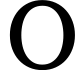
\includegraphics[width=0.5\textwidth,height=\textheight]{images/letter-O-150-dpi.png}
\caption{Raster graphics image of the letter O (150 dots per inch (dpi)
PNG format).}\label{fig:raster}
}
\end{figure}

\begin{figure}
\hypertarget{fig:vector}{%
\centering
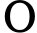
\includegraphics[width=0.5\textwidth,height=\textheight]{images/letter-O.svg}
\caption{Vector graphics image of the letter O (SVG
format).}\label{fig:vector}
}
\end{figure}

\hypertarget{raster-graphics}{%
\subsection{Raster Graphics}\label{raster-graphics}}

There are dozens of image formats, including these three major ones:

\begin{enumerate}
\tightlist
\item
  \href{https://en.wikipedia.org/wiki/TIFF}{Tag(ged) Image File Format
  (TIFF)}

  \begin{itemize}
  \tightlist
  \item
    lossless compression
  \item
    large file sizes
  \item
    used in printing and professional graphics
  \item
    preferred for archival of scanned photographs
  \end{itemize}
\item
  \href{https://jpeg.org/about.html}{Joint Photographic Experts Group
  (JPEG)} format

  \begin{itemize}
  \tightlist
  \item
    small file sizes
  \item
    lossy compression
  \item
    good quality with fast downloads
  \item
    supported by web browsers
  \item
    preferred for scenes and portraits
  \item
    no transparency
  \end{itemize}
\item
  \href{http://www.libpng.org/pub/png/}{Portable Network Graphics (PNG)}
  format

  \begin{itemize}
  \tightlist
  \item
    lossless compression
  \item
    preferred for text and high definition images
  \item
    supported by most web browsers
  \item
    transparency
  \end{itemize}
\end{enumerate}

All three formats yield images displayed as rectangular arrays of
\href{https://en.wikipedia.org/wiki/Pixels}{\emph{pixels}}.

\hypertarget{from-pictures-to-pixels}{%
\subsubsection{From pictures to pixels}\label{from-pictures-to-pixels}}

Imagine a picture on a square canvas being converted into a jig-saw
puzzle, only this time with square-shaped rather than irregular pieces.
If the picture were divided into a hundred pieces in one direction and
another hundred pieces in an
\href{https://en.wikipedia.org/wiki/Orthogonality}{orthogonal}
direction, we would have 100\textsuperscript{2} = 10,000 pieces in our
jig-saw puzzle. Each piece is a \emph{picture element} or \emph{pixel}
contributing to the overall picture.

Digital pictures are much the same, except for one difference. Whereas
each jig-saw puzzle piece carries a small, detailed part of the big
picture, each pixel consists of only \emph{one} colour. \emph{Pixels are
coloured tiles in a picture mosaic. Each tile contributes to the overall
picture, but it carries not a small picture, but a single colour}.

Clearly, the more tiles we have, the more detailed the emergent picture.
Conversely, if the entire picture were composed of a single tile, we
would see not a picture but a square of a single colour. Information has
been lost and we would have no idea what the picture was about, save for
that one dominant colour.

This possibility of information loss on converting an analog picture
into digital form is why, when we scan an image, we should take care to
digitize the picture with sufficient detail so that it represents the
original with fidelity.

\hypertarget{file-size-quality-and-compression}{%
\subsubsection{File size, quality, and
compression}\label{file-size-quality-and-compression}}

All raster images are rectangular arrays of pixels. How many pixels in
the \emph{width} and \emph{height} directions depends on how the
original analog image was scanned. Suppose the original image was
captured by a mobile phone, and thus already in digital form. If the
phone boasts of a 16 million pixel camera, we have a square image of
side \(\sqrt{16\times 10^6} = 4000\) pixels on each side.

While such an image would be incredibly detailed, it is
inconvenient---because of its large file size---for transmission on
social media or for display on the Web. The picture would have to be
\emph{resized} to smaller dimensions to yield a more manageable image
file size that still represents the original picture with fidelity. This
tradeoff between file size and visual quality or definition is at the
heart of digital image manipulation and format conversion.

It should be clear by now that we cannot tack a specific number of
pixels onto a digital image and say that is its one and only size.
Rather the number of pixels representing the width and height of a
picture are \emph{one digital representation} of the original analog
image. We may \emph{derive} another equally meaningful digital
representation by judiciously resizing the image to have a different
number of pixels in the width and height directions, while at the same
time yielding a more tractable file size, without loss of visual
quality.

Some image file formats are amenable to compression, which further
reduces file size. Certain formats are capable only of lossless
compression, leading to files that are slow to load, but with no loss of
information. Others allow lossy compression, where file size reduction
results in faster loading, but accompanied by loss of information. Why a
specific file format is used, and with what parameters, is determined by
image content, purpose, and application domain.

\hypertarget{pixel-densities-and-such}{%
\subsubsection{Pixel densities and
such}\label{pixel-densities-and-such}}

Raster images have a size denoted by the number of pixels comprising the
\emph{width} and \emph{height} of the image. The actual
\emph{dimensions} of the displayed image, however, depend on the
resolution of the display device.

Such images appear better defined at higher resolutions or pixel
densities. The units of resolution, or density, commonly used are
\emph{dots per inch} (dpi)---in the context of printers---or
\emph{pixels per inch} (ppi)---in the context of displays---both of
which reference the number of dots or pixels that may be accommodated in
one linear inch. It is possible to specify these in dots per centimetre,
or pixels per centimetre, but that usage has not caught on.

Commonly used resolutions for output devices are:

\begin{itemize}
\tightlist
\item
  72 ppi for low resolution monitors
\item
  96 ppi for standard resolution monitors
\item
  150 dpi/ppi\footnote{We will use dpi and ppi interchangeably hereafter
    to avoid inelegant expressions.}, which is often the default value
  in image conversion programs
\item
  300 dpi/ppi for some mobile phones and laser printers
\item
  600 dpi/ppi for higher end mobile phones and laser printers
\end{itemize}

Suppose we have an image that is a square of side 100 pixels. Its width
and height are each 100 pixels, and the image consists of a square array
of 100\textsuperscript{2} or 10,000 pixels. On a display that has a
resolution of 96 dpi, such an image will take up
\textsuperscript{100}/\textsubscript{96} = 1.042 inches on each side. If
the same image were displayed on a 300 dpi output device, its image will
span \textsuperscript{100}/\textsubscript{300} = 0.333 inches on each
side. Image sizes in pixels are therefore quite different from displayed
image dimensions in inches.

\begin{quote}
A pixel has no size, no physical value or meaning outside of its
mathematical representation.

\ldots{}

A pixel in itself has no size or physical representation, it can only
carry value through its relationship with the screen physical size,
creating the resolution, or PPI. Understand this and screen density will
have no secret for you. \protect\hyperlink{ref-gabriel2017}{{[}1{]}}
\end{quote}

\hypertarget{file-size-and-quality-again}{%
\subsubsection{File size and quality
again}\label{file-size-and-quality-again}}

If an image were resized to \emph{twice} its dimensions, the number of
pixels in it will become \emph{fourfold} as will, roughly, its file
size.

When photographic images are scanned, higher pixel densities lead to
much larger file sizes, resulting in images of remarkable detail.
Conversely, low resolution scans sacrifice image quality for small file
size. Good visual quality at reasonable file size is the much
sought-after optimal goal for any image.

Blocky images arise when the zoomed image is not matched to the display
resolution, allowing individual pixels to show themselves as discernible
``blocky'' elements, as in \cref{fig:raster}.

The dpi/ppi used for format conversion, especially between raster and
PDF, is critical to avoid getting ``blurry'' or ``grungy-looking''
images. Merely ratcheting up the source dpi/ppi before conversion from
raster to PDF will result in bloated PDF files that convey no
discernible improvement in visual quality. There is always a sweet spot
for pixel density---in image scanning and format conversions---that
gives good visual quality at a decent file size. We should aim for that.

\hypertarget{vector-graphics}{%
\subsection{Vector Graphics}\label{vector-graphics}}

The two principal vector graphics formats are:

\begin{enumerate}
\tightlist
\item
  \href{https://en.wikipedia.org/wiki/PDF}{Portable Document Format
  (PDF)}

  \begin{itemize}
  \tightlist
  \item
    preferred for archival quality electronic and printed documents
  \item
    supported by browsers with integrated PDF readers
  \item
    file sizes comparable to raster images
  \item
    machine-readable files
  \end{itemize}
\item
  \href{https://en.wikipedia.org/wiki/Scalable_Vector_Graphics}{Scalable
  Vector Graphics (SVG)} format

  \begin{itemize}
  \tightlist
  \item
    preferred for scalable graphics on web browsers
  \item
    used in digital image animations and digital art
  \item
    small file sizes
  \item
    human- and machine-readable files
  \end{itemize}
\end{enumerate}

Both these formats yield images which consist of mathematically defined
points, lines, curves, and shapes, which do not degrade in visual
quality when magnified.

\hypertarget{page-size-and-viewbox}{%
\subsubsection{Page size and viewBox}\label{page-size-and-viewbox}}

A raster image has a \emph{width} and a \emph{height} that are directly
related to the number of pixels in those two orthogonal directions.
Vector images, on the other hand, do not embody an intrinsic resolution,
and may therefore be zoomed in or out arbitrarily without loss of
detail. But vector images \emph{do have} intrinsic sizes that endow them
with a fixed \href{https://en.wikipedia.org/wiki/Aspect_ratio}{aspect
ratio}, no less than raster images.

The PDF format was developed for documents meant to be printed on paper.
It therefore embodies an intrinsic \emph{page size} in
\href{https://en.wikipedia.org/wiki/Point_(typography)}{points}, where
one point is \textsuperscript{1}/\textsubscript{72} of an inch. Points
are absolute linear dimensions which do not change with magnification.
In the PDF format, each graphic unit is paginated to the page size
parameter in points defined in the file.

With an image format that is designed primarily for display on the Web
via a Web browser---as is the case with SVG---image size is defined in
terms of a
\href{https://developer.mozilla.org/en-US/docs/Web/SVG/Attribute/viewBox}{\emph{viewBox}}.
The latter are again measured in points, and have a fixed
\href{https://en.wikipedia.org/wiki/Aspect_ratio}{aspect ratio},
determined by the image. Although such an SVG image may be zoomed
without loss of visual quality when displayed on the Web, it too has
intrinsic dimensions in terms of its viewBox.

The fact that raster images use pixels, which are relative to an image
array, and vector images use points, which are an absolute linear
measure, must be kept in mind during format conversion, to avoid
perplexing results after conversion.

\hypertarget{format-conversions}{%
\subsection{Format conversions}\label{format-conversions}}

For many reasons, it is often necessary to convert from one image format
to another. There are four broad possibilities for this, as shown below,
with typical examples:

\begin{enumerate}
\tightlist
\item
  Raster to raster: PNG to JPEG and vice versa;
\item
  Raster to vector: PNG to PDF or PNG to SVG;
\item
  Vector to raster: PDF to PNG or SVG to PNG; and
\item
  Vector to vector: PDF to SVG, or vice versa.
\end{enumerate}

We consider each of these in turn using
\href{https://itlaw.wikia.org/wiki/Platform_neutral}{platform-neutral}
\href{https://opensource.com/resources/what-open-source}{open source}
tools. Since I run
\href{https://en.wikipedia.org/wiki/GNU/Linux_naming_controversy}{GNU/Linux}
on my desktop, my examples will feature commands from that
setup.\footnote{There are many websites that promise conversion online,
  requiring you to upload the input file and download the output file.
  These \emph{might be} fraught with security risks. Use them with
  caution.}

\hypertarget{tools-for-image-format-conversion}{%
\subsection{Tools for image format
conversion}\label{tools-for-image-format-conversion}}

Among the very many tools available, we examine below four that support
image format conversion:

\begin{enumerate}
\tightlist
\item
  \href{https://imagemagick.org/index.php}{\texttt{ImageMagick}}

  \begin{itemize}
  \tightlist
  \item
    versatile graphics library for image manipulation and display
  \item
    standalone utilities like \texttt{convert}, \texttt{display},
    \texttt{identify}, \texttt{mogrify}, etc.
  \item
    scripting language support
  \item
    pixel-based
  \item
    raster to raster conversions
  \item
    raster to vector conversions
  \end{itemize}
\item
  \href{https://www.cairographics.org/}{cairo}

  \begin{itemize}
  \tightlist
  \item
    vector-based 2D drawing and rendering library
  \item
    multiple output devices/formats
  \item
    used by other programs as a backend, rather than in standalone mode
  \end{itemize}
\item
  \href{https://poppler.freedesktop.org/}{poppler}

  \begin{itemize}
  \tightlist
  \item
    vector-based PDF rendering library
  \item
    used by several PDF viewers
  \item
    uses cairo as backend
  \item
    standalone utilities like \texttt{pdftotext}, \texttt{pdftocairo},
    and \texttt{pdftoppm}
  \end{itemize}
\item
  \href{https://inkscape.org/}{Inkscape}

  \begin{itemize}
  \tightlist
  \item
    GUI-based vector graphics editor
  \item
    suitable both for technical illustration and digital art
  \item
    uses SVG as the working format
  \item
    can export to a wide variety of output formats
  \item
    option to use cairo for export to raster formats
  \end{itemize}
\end{enumerate}

\hypertarget{imagemagick-the-swiss-army-knife}{%
\subsection{\texorpdfstring{\texttt{ImageMagick}: the Swiss Army
knife}{ImageMagick: the Swiss Army knife}}\label{imagemagick-the-swiss-army-knife}}

\texttt{ImageMagick} is the name given to a suite of image processing
tools originally created in 1987 by John Cristy, then working for
\href{https://www.dupont.com/}{Du Pont}. In 1990, it was freely released
by Du Pont, who transferred copyright to
\href{https://imagemagick.org/script/contact.php}{ImageMagick Studio
LLC} who now maintain the project. It is distributed under a
\href{https://imagemagick.org/script/license.php}{derived Apache 2.0
license}. The
\href{https://github.com/ImageMagick/ImageMagick}{authoritative source
code repository} shows active development even today, 34 years after the
suite was first released
\protect\hyperlink{ref-imagemagicksource}{{[}2{]}}.

\texttt{ImageMagick} is so versatile and useful that it may rightfully
be called the
\href{https://www.thefreedictionary.com/Swiss-army+knife}{Swiss Army
knife} of the image processing world. It comes with several command line
utilities, each replete with options. Among these are:

\begin{itemize}
\tightlist
\item
  \href{https://imagemagick.org/script/convert.php}{\texttt{convert}}
  which converts from one format to another;
\item
  \href{https://imagemagick.org/script/display.php}{\texttt{display}}
  which displays one or more images;
\item
  \href{https://imagemagick.org/script/identify.php}{\texttt{identify}}
  which identifies the type of image and displays its characteristics;
\item
  \href{https://imagemagick.org/script/mogrify.php}{\texttt{mogrify}}
  which transforms an image, modifying its appearance; and
\item
  \href{https://imagemagick.org/script/montage.php}{\texttt{montage}}
  which generates an image montage from several images.
\end{itemize}

The above list is far from exhaustive. The interested reader is referred
to the
\href{https://imagemagick.org/script/command-line-tools.php}{excellent
online documentation} for further details. The power of
\texttt{ImageMagick} is enhanced with the
\href{https://imagemagick.org/script/magick-script.php}{magick-script}
Image Scripting Language. The examples in this blog use the command line
versions of invoking \texttt{ImageMagick}. If they seem daunting,
\href{https://imagemagick.org/script/command-line-processing.php}{refer
to this explanation} \protect\hyperlink{ref-imcli}{{[}3{]}}.

\hypertarget{test-images}{%
\subsection{Test images}\label{test-images}}

Two quite different images are used to illustrate the format conversions
we perform here. The two test images are:

\begin{enumerate}
\tightlist
\item
  a coloured, text-only test image contained in the file
  \href{images/text-only.pdf}{\texttt{text-only.pdf}}; and
\item
  a coloured, non-text, graphically rich image contained in the file
  \href{images/animals.jpg}{\texttt{animals.jpg}}.
\end{enumerate}

We will succinctly refer to these two images as \texttt{text-only} and
\texttt{animals}, respectively hereafter.

\hypertarget{the-text-only-image}{%
\subsubsection{\texorpdfstring{The \texttt{text-only}
image}{The text-only image}}\label{the-text-only-image}}

The text-only image was first generated programmatically as a PDF file,
\texttt{text-only.pdf}, by compiling a
\href{https://www.latex-project.org/}{LaTeX}
\href{auxiliary/text-only.tex}{source file}. PDF is the \emph{native} or
natural format for this image. The \texttt{text-only} image converted
into any other format must be measured against the benchmark of the
original PDF in file size and visual quality.

PDFs may be displayed on \emph{separate} browser tabs, but cannot be
displayed, among other content, \emph{within} a web page.
\href{images/text-only.pdf}{Click here} to see \texttt{text-only.pdf} as
a zoomable PDF on a separate browser tab.

\hypertarget{converting-text-only-from-pdf-to-png-and-jpeg}{%
\paragraph{\texorpdfstring{Converting \texttt{text-only} from PDF to PNG
and
JPEG}{Converting text-only from PDF to PNG and JPEG}}\label{converting-text-only-from-pdf-to-png-and-jpeg}}

To display \texttt{text-only} on this page, the original PDF file was
converted to the PNG and JPEG formats using the methods
\protect\hyperlink{vector-to-raster}{discussed later} to yield the
raster images \texttt{text-only-600-dpi-cairo.png} and
\texttt{text-only-600-dpi-cairo.jpg}. The commands we used are shown
below for completeness, but
\protect\hyperlink{pdf-to-png-and-jpeg-poppler-and-cairo}{explained
later}:

\begin{Shaded}
\begin{Highlighting}[]
\CommentTok{\# PDF to PNG at 600 dpi}
\ExtensionTok{pdftocairo} \AttributeTok{{-}png} \AttributeTok{{-}r}\NormalTok{ 600 }\AttributeTok{{-}singlefile} \DataTypeTok{\textbackslash{}}
\NormalTok{text{-}only.pdf text{-}only{-}600{-}dpi{-}cairo}

\CommentTok{\# PDF to lossless JPEG at 600 dpi}
\ExtensionTok{pdftocairo} \AttributeTok{{-}jpeg} \AttributeTok{{-}jpegopt}\NormalTok{ quality=100 }\AttributeTok{{-}r}\NormalTok{ 600 }\AttributeTok{{-}singlefile} \DataTypeTok{\textbackslash{}}
\NormalTok{text{-}only.pdf text{-}only{-}600{-}dpi{-}cairo}
\end{Highlighting}
\end{Shaded}

\begin{figure}
\hypertarget{fig:text-only-png-cairo}{%
\centering

\includegraphics[width=0.8\textwidth,height=\textheight]{images/text-only-600-dpi-cairo.png}
\caption{Text-only image in 600 dpi PNG
format.}\label{fig:text-only-png-cairo}
}
\end{figure}

\begin{figure}
\hypertarget{fig:text-only-jpg-cairo}{%
\centering

\includegraphics[width=0.8\textwidth,height=\textheight]{images/text-only-600-dpi-cairo.jpg}
\caption{Text-only image in 600 dpi lossless JPEG
format.}\label{fig:text-only-jpg-cairo}
}
\end{figure}

\hypertarget{file-sizes}{%
\paragraph{File sizes}\label{file-sizes}}

\begin{Shaded}
\begin{Highlighting}[]
\FunctionTok{ls} \AttributeTok{{-}Xsh}\NormalTok{ text{-}only.pdf text{-}only{-}600{-}dpi{-}cairo.}\PreprocessorTok{*} \KeywordTok{|} \DataTypeTok{\textbackslash{}}
\FunctionTok{awk} \StringTok{\textquotesingle{}\{print $1 "\textbackslash{}t" $2\}\textquotesingle{}}
\ExtensionTok{{-}{-}{-}}
\ExtensionTok{120K}\NormalTok{    text{-}only{-}600{-}dpi{-}cairo.jpg}
\ExtensionTok{16K}\NormalTok{     text{-}only.pdf}
\ExtensionTok{40K}\NormalTok{     text{-}only{-}600{-}dpi{-}cairo.png}
\end{Highlighting}
\end{Shaded}

As a convention hereafter, when there is a \texttt{-\/-\/-} separator
between a command and some results, the latter are the results displayed
on execution of the command.

The file sizes are displayed above merely for information. Note that the
JPEG file is an order of magnitude larger than both the original PDF and
the PNG. The relative strengths and weaknesses of different file formats
for displaying different image types are discussed later.

\hypertarget{the-animals-image}{%
\subsubsection{\texorpdfstring{The \texttt{animals}
image}{The animals image}}\label{the-animals-image}}

The non-text \texttt{animals.jpg} image is a cropped version of the
original image \texttt{animals-original.jpg}
\href{https://www.rawpixel.com/image/2266608/free-illustration-image-ernst-haeckel-vintage-animals}{downloaded
from the Web}. It is a colourful, graphically rich image with much
detail, and is from a hand-drawn illustration of microscopic marine
animals by the German naturalist
\href{https://en.wikipedia.org/wiki/Ernst_Haeckel}{Ernst Haeckel},
scanned as a JPEG, and made available in the public domain.

Note that \texttt{animals-original.jpg} has been scanned from a printed,
hard copy illustration and saved as a JPEG raster file. That is its
native format. All conversions should be gauged against the file size
and visual quality of the cropped original \texttt{animals.jpg}.

\begin{figure}
\hypertarget{fig:animals-original}{%
\centering
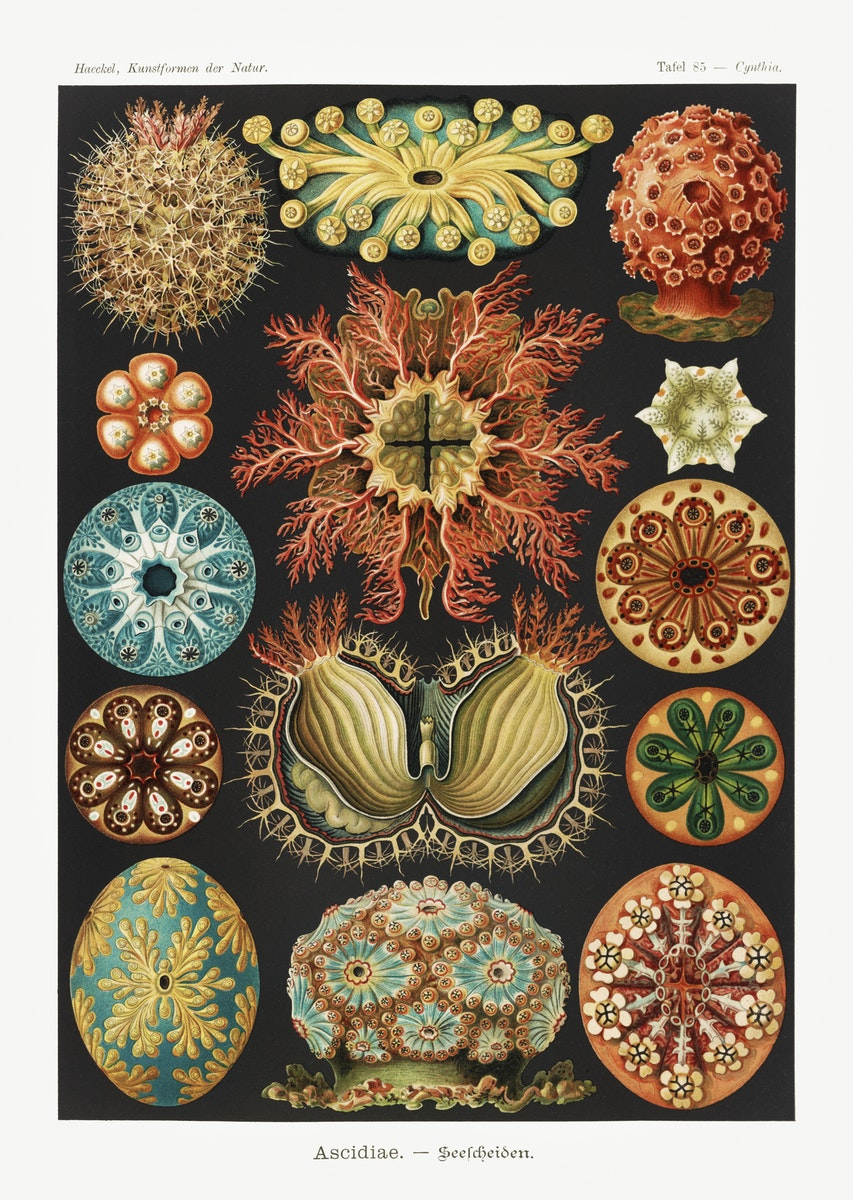
\includegraphics[width=0.8\textwidth,height=\textheight]{images/animals-original.jpg}
\caption[Non-text, graphically rich \texttt{animals-original.jpg} image
in JPEG format.]{Non-text, graphically rich
\texttt{animals-original.jpg} image in JPEG
format.\footnotemark{}}\label{fig:animals-original}
}
\end{figure}
\footnotetext{These images are in the public domain and covered by the
  \href{https://creativecommons.org/publicdomain/zero/1.0/}{CC0
  licence}.}

How the original image was cropped to get the \texttt{animals} image is
explained next.

\hypertarget{pre-processing-animals}{%
\paragraph{\texorpdfstring{Pre-processing
\texttt{animals}}{Pre-processing animals}}\label{pre-processing-animals}}

Cropping is strictly not image format conversion, but is often a
necessary pre-processing step in image manipulations. For example,
\cref{fig:animals-original} has a whitish, non-monochromatic border
around the block print, containing annotations. For our purposes, this
border is at best a distraction. It may be removed altogether by
\emph{cropping}, leaving us with only the illustration. The resulting
cropped image, \texttt{animals.jpg} will be the source image in our
examples below.

\hypertarget{cropping}{%
\paragraph{Cropping}\label{cropping}}

Cropping is usually better done interactively using a
\href{https://en.wikipedia.org/wiki/Graphical_user_interface}{GUI
(Graphical User Interface)}, than on the command line. However, the
latter, even if a bit tedious, is precisely repeatable.

The \texttt{display} utility of \texttt{ImageMagick} pops up a GUI,
shown in \cref{fig:gui}, when the mouse is over the image and the left
mouse button is clicked. We can then drag and fit a window to the
\emph{region we wish to keep}, clicking the \texttt{Crop} function, and
saving the cropped image. The steps are these:

\begin{enumerate}
\def\labelenumi{\alph{enumi}.}
\tightlist
\item
  left mouse click on the image to reveal the GUI;
\item
  \texttt{Transform\ -\textgreater{}\ Crop};
\item
  put the mouse over the top left corner and drag until the bottom right
  corner to enclose the region of interest;
\item
  Click again on \texttt{Crop}; and
\item
  \texttt{File\ -\textgreater{}\ Save} with a different name.
\end{enumerate}

\begin{figure}
\hypertarget{fig:gui}{%
\centering
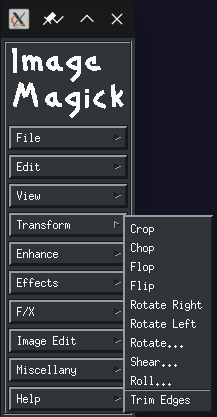
\includegraphics[width=0.3\textwidth,height=\textheight]{images/ImageMagick-display-gui.png}
\caption{\texttt{ImageMagick} interactive GUI.}\label{fig:gui}
}
\end{figure}

Alternatively, we may just position the cursor on the top left and
bottom right corners of the region we wish to \emph{retain}, noting the
co-ordinates in each case. If these coordinates are \((x_t, y_t)\) and
\((x_b, y_b)\), respectively, we have \(w = x_b - x_t\) and
\(h = y_b -y_t\). We may then invoke the convert command with crop as
the option so:

\begin{Shaded}
\begin{Highlighting}[]
\ExtensionTok{convert} \AttributeTok{{-}crop} \StringTok{\textquotesingle{}wxh+x\_t+y\_t\textquotesingle{}}\NormalTok{ animals{-}original.jpg animals.jpg}
\end{Highlighting}
\end{Shaded}

In our case, \((x_t, y_t) = (60, 84)\) and \((x_b, y_b) = (795, 1119)\)
giving \(w = 735\) and \(h = 1035\), leading to

\begin{Shaded}
\begin{Highlighting}[]
\ExtensionTok{convert} \AttributeTok{{-}crop} \StringTok{\textquotesingle{}735x1035+60+84\textquotesingle{}}\NormalTok{ animals{-}original.jpg animals.jpg}
\end{Highlighting}
\end{Shaded}

The resulting cropped image, \texttt{animals.jpg} is shown in
\cref{fig:cropped} below.

\begin{figure}
\hypertarget{fig:cropped}{%
\centering
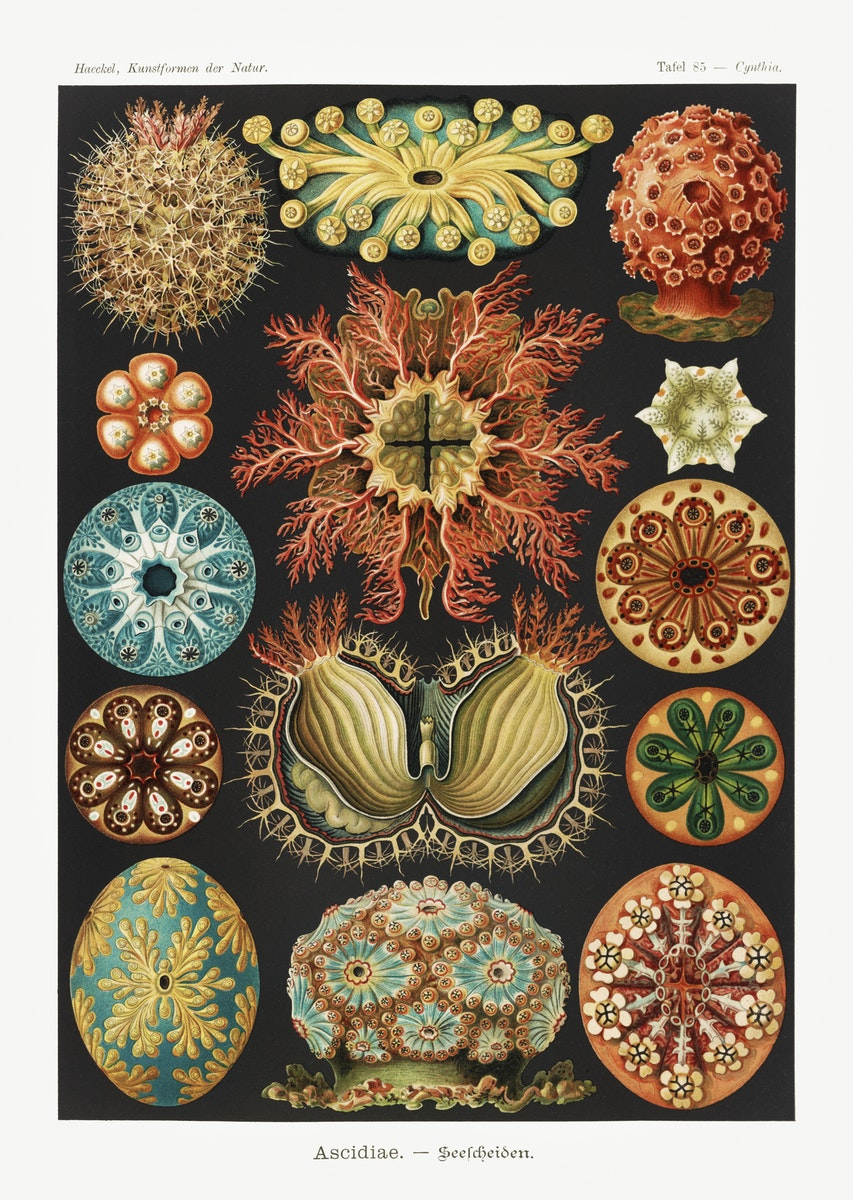
\includegraphics[width=0.5\textwidth,height=\textheight]{images/animals.jpg}
\caption{Cropped version of the original image in
\cref{fig:animals-original}. This is the \texttt{animals.jpg}
image.}\label{fig:cropped}
}
\end{figure}

\hypertarget{file-sizes-1}{%
\paragraph{File sizes}\label{file-sizes-1}}

The sizes of the original and cropped files are shown below in human
friendly numbers:

\begin{Shaded}
\begin{Highlighting}[]
\FunctionTok{ls} \AttributeTok{{-}Xsh}\NormalTok{ animals}\PreprocessorTok{*}\NormalTok{.jpg }\KeywordTok{|} \FunctionTok{awk} \StringTok{\textquotesingle{}\{print $1 "\textbackslash{}t" $2\}\textquotesingle{}}
\ExtensionTok{{-}{-}{-}}
\ExtensionTok{200K}\NormalTok{    animals.jpg}
\ExtensionTok{312K}\NormalTok{    animals{-}original.jpg}
\end{Highlighting}
\end{Shaded}

As expected, the original file \texttt{animals-original.jpg} is larger
than the cropped full-size version, \texttt{animals.jpg}, and all is
well.

\hypertarget{raster-to-raster-conversion}{%
\subsection{Raster to raster
conversion}\label{raster-to-raster-conversion}}

We now perform a sequence of image manipulations, including raster to
raster format conversions.

\hypertarget{resizing-format-conversion-and-montaging}{%
\subsubsection{Resizing, format-conversion, and
montaging}\label{resizing-format-conversion-and-montaging}}

We may invoke the \texttt{convert} function of \texttt{ImageMagick} not
only to convert from one format to another but also to accomplish
cropping (as we have already seen), image-resizing, making the
background transparent, and
\href{https://www.thefreedictionary.com/montage}{montaging}, etc.

Suppose we want to reduce the dimensions of the cropped image to half
their original values, and display the full-size and half-size images
side by side, we could run the following command:

\begin{Shaded}
\begin{Highlighting}[]
\ExtensionTok{convert}\NormalTok{ animals.jpg }\AttributeTok{{-}resize}\NormalTok{ 50\% animals{-}halfsize.jpg}

\CommentTok{\# Composite the two images by aligning their bottoms}
\ExtensionTok{convert}\NormalTok{ +append }\AttributeTok{{-}gravity}\NormalTok{ south }\DataTypeTok{\textbackslash{}}
\NormalTok{animals.jpg animals{-}halfsize.jpg animals{-}both.jpg}
\end{Highlighting}
\end{Shaded}

\begin{figure}
\hypertarget{fig:animals-both-jpg}{%
\centering
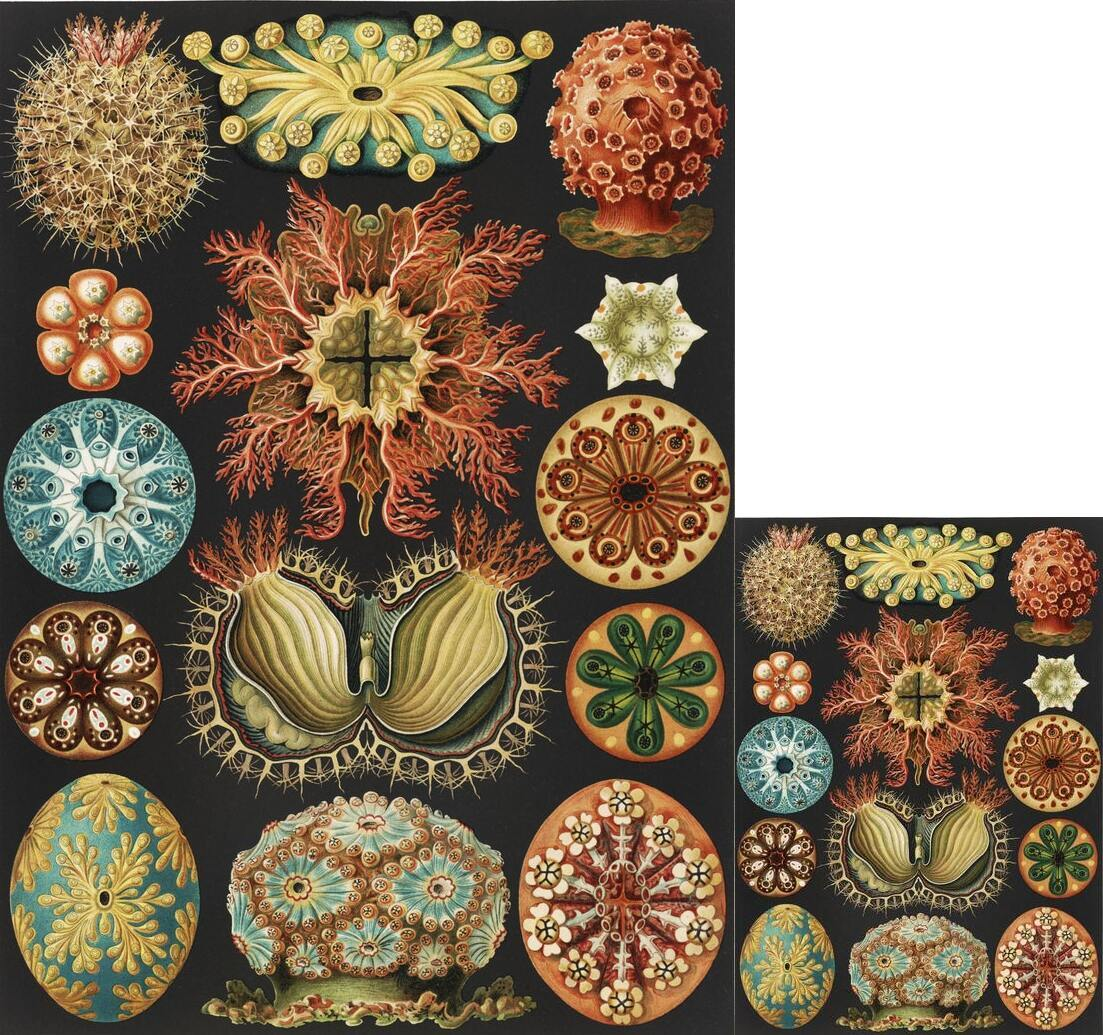
\includegraphics[width=0.8\textwidth,height=\textheight]{images/animals-both.jpg}
\caption{Full-size cropped image on the left and half-sized image on the
right in JPEG format.}\label{fig:animals-both-jpg}
}
\end{figure}

\hypertarget{background-transparency}{%
\subsubsection{Background transparency}\label{background-transparency}}

Notice that there is a coloured white rectangle atop the half-size image
on the right in \cref{fig:animals-both-jpg}. We could remove it by
rendering the background transparent. However, because JPEG does not
support transparency (through an
\href{https://www.techopedia.com/definition/1945/alpha-channel}{alpha
channel}) we have to convert the composite image to the PNG format,
which does support transparency. This is an example of why we need to
convert from one format to another.

\begin{Shaded}
\begin{Highlighting}[]
\CommentTok{\# Non{-}transparent composite in PNG}
\ExtensionTok{convert}\NormalTok{ +append }\AttributeTok{{-}gravity}\NormalTok{ south }\DataTypeTok{\textbackslash{}}
\NormalTok{animals.jpg animals{-}halfsize.jpg animals{-}both{-}non{-}transparent.png}

\CommentTok{\# Transparent composite in PNG}
\ExtensionTok{convert}\NormalTok{ +append }\AttributeTok{{-}gravity}\NormalTok{ south }\AttributeTok{{-}background}\NormalTok{ transparent }\DataTypeTok{\textbackslash{}}
\NormalTok{animals.jpg animals{-}halfsize.jpg animals{-}both{-}transparent.png}
\end{Highlighting}
\end{Shaded}

\begin{figure}
\hypertarget{fig:animals-both-transparent-png}{%
\centering
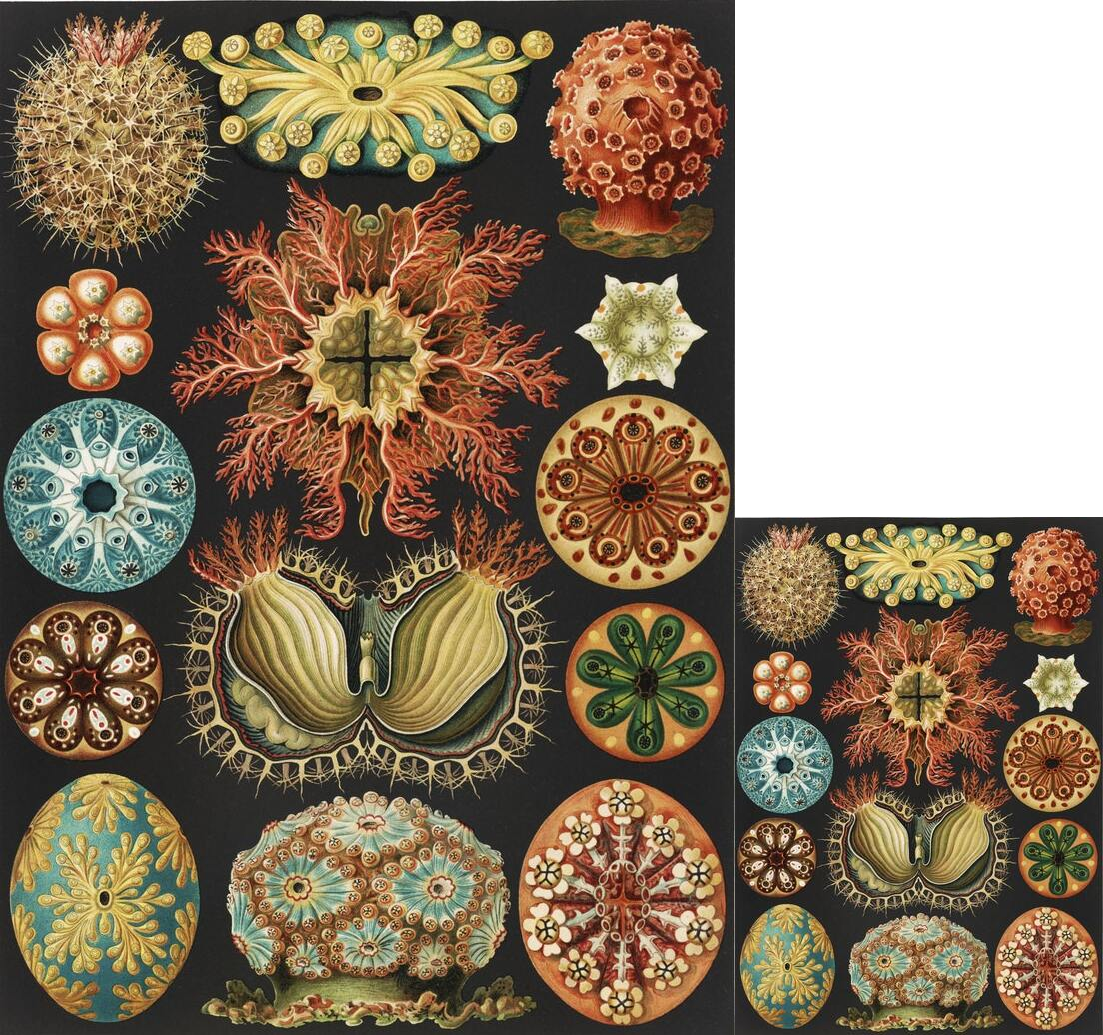
\includegraphics[width=0.8\textwidth,height=\textheight]{images/animals-both-transparent.png}
\caption{Composite image converted to PNG format with transparent
background.}\label{fig:animals-both-transparent-png}
}
\end{figure}

\hypertarget{file-sizes-again}{%
\paragraph{File sizes again}\label{file-sizes-again}}

How do the file sizes of the three composite images compare? How does
the non-transparent JPEG compare with the non-transparent PNG? Also, how
high a price have we paid for the transparent background?

\begin{Shaded}
\begin{Highlighting}[]
\FunctionTok{ls} \AttributeTok{{-}Xsh}\NormalTok{ animals{-}both}\PreprocessorTok{*}\KeywordTok{|} \FunctionTok{awk} \StringTok{\textquotesingle{}\{print $1 "\textbackslash{}t" $2\}\textquotesingle{}}
\ExtensionTok{{-}{-}{-}}
\ExtensionTok{264K}\NormalTok{    animals{-}both.jpg}
\ExtensionTok{2.0M}\NormalTok{    animals{-}both{-}non{-}transparent.png}
\ExtensionTok{2.2M}\NormalTok{    animals{-}both{-}transparent.png}
\end{Highlighting}
\end{Shaded}

The PNG composite image is \emph{more than seven times larger} than its
JPEG counterpart, \emph{even without transparency}. And transparency
makes the PNG file size ten percent larger.

\hypertarget{compression-levels-and-file-sizes}{%
\paragraph{Compression levels and file
sizes}\label{compression-levels-and-file-sizes}}

The \href{https://en.wikipedia.org/wiki/Image_compression}{image
compression level} used above is the default compression level in
\texttt{ImageMagick}. Getting the right combination of image format,
image dimensions, image compression, and image quality so that the image
loads fast and looks good is
\href{https://www.smashingmagazine.com/2015/06/efficient-image-resizing-with-imagemagick/}{quite
an art}. \protect\hyperlink{ref-newton2015}{{[}4{]}}

To get an idea of the range of file sizes involved, let us try
generating a composite image with extremes of the compression level,
which can range from 0 to 9.

\begin{Shaded}
\begin{Highlighting}[]
\CommentTok{\# Least compression}
\ExtensionTok{convert} \AttributeTok{{-}define}\NormalTok{ PNG:compression{-}level=0 +append }\AttributeTok{{-}gravity}\NormalTok{ south }\DataTypeTok{\textbackslash{}}
\NormalTok{{-}background transparent }\DataTypeTok{\textbackslash{}}
\NormalTok{animals.jpg animals{-}halfsize.jpg }\DataTypeTok{\textbackslash{}}
\NormalTok{animals{-}both{-}compressed{-}0.png}

\CommentTok{\# Most compression}
\ExtensionTok{convert} \AttributeTok{{-}define}\NormalTok{ PNG:compression{-}level=9 +append }\AttributeTok{{-}gravity}\NormalTok{ south }\DataTypeTok{\textbackslash{}}
\NormalTok{{-}background transparent }\DataTypeTok{\textbackslash{}}
\NormalTok{animals.jpg animals{-}halfsize.jpg }\DataTypeTok{\textbackslash{}}
\NormalTok{animals{-}both{-}compressed{-}9.png}
\end{Highlighting}
\end{Shaded}

The file sizes are:

\begin{Shaded}
\begin{Highlighting}[]
\FunctionTok{ls} \AttributeTok{{-}Xsh}\NormalTok{ animals{-}both}\PreprocessorTok{*} \KeywordTok{|} \FunctionTok{awk} \StringTok{\textquotesingle{}\{print $1 "\textbackslash{}t" $2\}\textquotesingle{}}
\ExtensionTok{{-}{-}{-}}
\ExtensionTok{264K}\NormalTok{    animals{-}both.jpg}
\ExtensionTok{4.4M}\NormalTok{    animals{-}both{-}compressed{-}0.png}
\ExtensionTok{2.2M}\NormalTok{    animals{-}both{-}compressed{-}9.png}
\ExtensionTok{2.0M}\NormalTok{    animals{-}both{-}non{-}transparent.png}
\ExtensionTok{2.2M}\NormalTok{    animals{-}both{-}transparent.png}
\end{Highlighting}
\end{Shaded}

It appears that the default compression used by \texttt{ImageMagick}
gives a file size that is the same as the highest compression level.
Indeed, the uncompressed version---with a compression level of
zero---gives a file \emph{twice} the size of the uncompressed version
and \emph{sixteen times} the size of the JPEG. And we have not even used
two other related attributes:
\href{https://stackoverflow.com/questions/27267073/imagemagick-lossless-max-compression-for-png}{filter
and strategy} \protect\hyperlink{ref-setchell2014}{{[}5{]}}. Getting the
best tradeoff of image format, image size, file size, loading time, and
image quality is still more of an art to be mastered than an algorithm
to be applied.

We may conclude from the above that non-textual, detail-rich images are
better stored and displayed as JPEGs than PNGs.

\hypertarget{results-with-text-only}{%
\subsubsection{\texorpdfstring{Results with
\texttt{text-only}}{Results with text-only}}\label{results-with-text-only}}

Recall that \texttt{text-only} was originally generated as a PDF.
\protect\hyperlink{converting-text-only-from-pdf-to-png-and-jpeg}{Previously},
we briefly touched upon how we converted \texttt{text-only} from PDF to
PNG and JPEG.

To get a PNG version of the image, we need to
\protect\hyperlink{pdf-to-png-and-jpeg-poppler-and-cairo}{run a little
ahead of ourselves and convert from PDF to PNG}.

From that PNG, let us do a simple \emph{no quality loss} conversion from
PNG to JPEG for \texttt{text-only}, and compare appearances and file
sizes.

\begin{Shaded}
\begin{Highlighting}[]
\CommentTok{\# Lossless JPEG with a \textquotesingle{}quality\textquotesingle{} of 100 from PNG}
\ExtensionTok{convert} \AttributeTok{{-}quality}\NormalTok{ 100 text{-}only{-}600{-}dpi{-}cairo.png }\DataTypeTok{\textbackslash{}}
\NormalTok{text{-}only{-}600{-}dpi{-}cairo{-}IM.jpg}

\CommentTok{\# Composite both images into one PNG with a transparent divider}
\ExtensionTok{convert}\NormalTok{ text{-}only{-}600{-}dpi{-}cairo.png text{-}only{-}600{-}dpi{-}cairo{-}IM.jpg }\DataTypeTok{\textbackslash{}}
\NormalTok{{-}background transparent }\AttributeTok{{-}splice}\NormalTok{ 20x0+0+0 +append }\AttributeTok{{-}chop}\NormalTok{ 20x0+0+0 }\DataTypeTok{\textbackslash{}}
\NormalTok{text{-}only{-}both{-}600{-}dpi{-}cairo.png}

\CommentTok{\# Composite both images into one JPEG with a transparent divider}
\ExtensionTok{convert}\NormalTok{ text{-}only{-}600{-}dpi{-}cairo.png text{-}only{-}600{-}dpi{-}cairo{-}IM.jpg }\DataTypeTok{\textbackslash{}}
\NormalTok{{-}background transparent }\AttributeTok{{-}splice}\NormalTok{ 20x0+0+0 +append }\AttributeTok{{-}chop}\NormalTok{ 20x0+0+0 }\DataTypeTok{\textbackslash{}}
\NormalTok{text{-}only{-}both{-}600{-}dpi{-}cairo.jpg}

\FunctionTok{ls} \AttributeTok{{-}Xsh}\NormalTok{ text{-}only{-}600{-}dpi{-}cairo.png }\DataTypeTok{\textbackslash{}}
\NormalTok{text{-}only{-}600{-}dpi{-}cairo{-}IM.jpg }\DataTypeTok{\textbackslash{}}
\NormalTok{text{-}only{-}both{-}600{-}dpi{-}cairo.}\PreprocessorTok{*} \DataTypeTok{\textbackslash{}}
\KeywordTok{|} \FunctionTok{awk} \StringTok{\textquotesingle{}\{print $1 "\textbackslash{}t" $2\}\textquotesingle{}}
\ExtensionTok{{-}{-}{-}}
\ExtensionTok{148K}\NormalTok{    text{-}only{-}600{-}dpi{-}cairo{-}IM.jpg}
\ExtensionTok{148K}\NormalTok{    text{-}only{-}both{-}600{-}dpi{-}cairo.jpg}
\ExtensionTok{40K}\NormalTok{     text{-}only{-}600{-}dpi{-}cairo.png}
\ExtensionTok{120K}\NormalTok{    text{-}only{-}both{-}600{-}dpi{-}cairo.png}
\end{Highlighting}
\end{Shaded}

\begin{figure}
\hypertarget{fig:text-only-both-png}{%
\centering

\includegraphics[width=0.8\textwidth,height=\textheight]{images/text-only-both-600-dpi-cairo.png}
\caption{Composite PNG image of the PNG on the left, and JPEG on the
right.}\label{fig:text-only-both-png}
}
\end{figure}

The right sub-image of \cref{fig:text-only-both-png} does not reveal
noticeable degradation in quality after conversion from PNG to JPEG, and
back to PNG again. Note also that the file size of the \emph{composite}
PNG image is smaller than the file size of the \emph{single} JPEG image.

\begin{figure}
\hypertarget{fig:text-only-both-jpg}{%
\centering

\includegraphics[width=0.8\textwidth,height=\textheight]{images/text-only-both-600-dpi-cairo.jpg}
\caption{Composite JPEG image of the PNG on the left, and JPEG on the
right.}\label{fig:text-only-both-jpg}
}
\end{figure}

Likewise, notice that when the composite image,
\cref{fig:text-only-both-jpg} is a JPEG, there is no noticeable
degradation in image quality. Moreover, the file size of the composite
is the same as for the singleton JPEG image. Note also that because JPEG
does not support transparency, the sliver of ``transparent background''
sandwiched between the two images now appears black.

\hypertarget{png-for-text-and-jpeg-for-non-text}{%
\subsubsection{PNG for text and JPEG for
non-text}\label{png-for-text-and-jpeg-for-non-text}}

We conclude from the \texttt{text-only} images that PNG is better suited
for textual images and provides a smaller file size for the same
quality.

Conversely, we know from the \texttt{animals} images that JPEG is more
suited to non-textual detail and yields good quality images at far
smaller file sizes than PNG.

\hypertarget{can-cairo-and-poppler-do-all-this}{%
\subsubsection{\texorpdfstring{Can \texttt{cairo} and \texttt{poppler}
do all
this?}{Can cairo and poppler do all this?}}\label{can-cairo-and-poppler-do-all-this}}

It is all a question of what format do we start with?

Both \texttt{cairo} and \texttt{poppler} are designed for PDF input
images. They stand out as tools of choice when we start off with PDFs.

The \texttt{animals} image, on the other hand, is scanned from an
illustration. Our input is a JPEG raster image. The forte of
\texttt{ImageMagick} is the display, manipulation, format conversion,
and processing of raster images. So, we run with the utilities provided
by \texttt{ImageMagick} in the latter case.

\hypertarget{raster-to-vector-conversions}{%
\subsection{Raster to vector
conversions}\label{raster-to-vector-conversions}}

Let us say that we have a logo, designed and available as a raster image
in some format. To use it on the Web, we could, if necessary, reformat
it as a JPEG or PNG file. But as we zoom into the page, the raster
images will start becoming less sharp and more blocky as shown in
\cref{fig:raster}.

However, if the graphic were in SVG format, supported by most web
browsers, the logo would scale without visual degradation as we zoom
into the page.

How do we convert a raster image to a vector format like PDF or SVG?

\hypertarget{raster-to-pdf-with-convert-for-animals}{%
\subsubsection{\texorpdfstring{Raster to PDF with \texttt{convert} for
\texttt{animals}}{Raster to PDF with convert for animals}}\label{raster-to-pdf-with-convert-for-animals}}

The \texttt{convert} utility of \texttt{ImageMagick} comes to our rescue
again. For example,

\begin{Shaded}
\begin{Highlighting}[]
\CommentTok{\# Convert JPEG image to PDF}
\ExtensionTok{convert}\NormalTok{ animals.jpg animals{-}IM.pdf}

\FunctionTok{ls} \AttributeTok{{-}Xsh}\NormalTok{ animals.jpg animals{-}IM.pdf }\KeywordTok{|} \FunctionTok{awk} \StringTok{\textquotesingle{}\{print $1 "\textbackslash{}t" $2\}\textquotesingle{}}
\ExtensionTok{{-}{-}{-}}
\ExtensionTok{200K}\NormalTok{    animals.jpg}
\ExtensionTok{204K}\NormalTok{    animals{-}IM.pdf}
\end{Highlighting}
\end{Shaded}

Web browsers, while they may feature PDF viewers on separate tabs, are
still unable to display PDFs as part of a web page. The converted image,
\href{images/animals-IM.pdf}{\texttt{animals-IM.pdf}}, may be viewed on
a browser tab from the given link. If the converted PDF is magnified by
zooming, it will be seen to reveal remarkable detail. And the difference
between the JPEG and PDF file sizes is negligible.

What happens, though, if the half-sized image is used to generate the
PDF? It is smaller and accordingly embodies less information than the
original, again commensurate with the respective file sizes.

\begin{Shaded}
\begin{Highlighting}[]
\ExtensionTok{convert}\NormalTok{ animals{-}halfsize.jpg animals{-}halfsize.pdf}

\FunctionTok{ls} \AttributeTok{{-}Xsh}\NormalTok{ animals{-}halfsize.jpg animals{-}halfsize.pdf }\KeywordTok{|} \DataTypeTok{\textbackslash{}}
\FunctionTok{awk} \StringTok{\textquotesingle{}\{print $1 "\textbackslash{}t" $2\}\textquotesingle{}}
\ExtensionTok{{-}{-}{-}}
\ExtensionTok{64K}\NormalTok{     animals{-}halfsize.jpg}
\ExtensionTok{64K}\NormalTok{     animals{-}halfsize.pdf}
\end{Highlighting}
\end{Shaded}

Increasing detail demands larger file sizes: there is no free lunch. But
the conversion from PDF to JPEG does not cost us much, if at all, in
file size.

\hypertarget{raster-to-svg-with-convert}{%
\subsubsection{\texorpdfstring{Raster to SVG with
\texttt{convert}}{Raster to SVG with convert}}\label{raster-to-svg-with-convert}}

Will \texttt{convert} cater for a JPEG to SVG conversion?

\begin{Shaded}
\begin{Highlighting}[]
\CommentTok{\# Original \textasciigrave{}animals.jpg\textasciigrave{} to SVG using \textasciigrave{}convert\textasciigrave{}}
\ExtensionTok{convert}\NormalTok{ animals.jpg animals{-}IM.svg}

\FunctionTok{ls} \AttributeTok{{-}Xsh}\NormalTok{ animals.jpg animals{-}IM.svg }\KeywordTok{|} \FunctionTok{awk} \StringTok{\textquotesingle{}\{print $1 "\textbackslash{}t" $2\}\textquotesingle{}}
\ExtensionTok{{-}{-}{-}}
\ExtensionTok{200K}\NormalTok{    animals.jpg}
\ExtensionTok{436K}\NormalTok{    animals{-}IM.svg}
\end{Highlighting}
\end{Shaded}

The SVG file is more than \emph{twice} the size of the original JPEG.
The question arises whether there is an alternative route to the SVG
that could give us smaller file sizes but comparable fidelity. What if
we did not convert from raster to SVG but from raster to PDF and thence
to SVG?

Since PDF to SVG conversion is really part of vector to vector
conversion, we will
\protect\hyperlink{pdf-to-svg-with-the-animals-image}{revisit this
question later}.

\hypertarget{round-tripping-from-pdf-through-png-to-pdf}{%
\subsubsection{Round tripping from PDF through PNG to
PDF}\label{round-tripping-from-pdf-through-png-to-pdf}}

The \texttt{text-only} image first saw life as a PDF. We then converted
it to a 600 dpi PNG. What happens if we convert that image back to a
PDF?

\begin{Shaded}
\begin{Highlighting}[]
\CommentTok{\# Generate PDF from 600 dpi PNG using \textasciigrave{}convert\textasciigrave{}}
\ExtensionTok{convert}\NormalTok{ text{-}only{-}600{-}dpi{-}cairo.png text{-}only{-}from{-}600{-}dpi{-}PNG.pdf}

\FunctionTok{ls} \AttributeTok{{-}Xsh}\NormalTok{ text{-}only}\PreprocessorTok{*}\NormalTok{600}\PreprocessorTok{*}\NormalTok{.pdf text{-}only.pdf }\KeywordTok{|} \FunctionTok{awk} \StringTok{\textquotesingle{}\{print $1 "\textbackslash{}t" $2\}\textquotesingle{}}
\ExtensionTok{{-}{-}{-}}
\ExtensionTok{40K}\NormalTok{     text{-}only{-}from{-}600{-}dpi{-}PNG.pdf}
\ExtensionTok{16K}\NormalTok{     text{-}only.pdf}
\end{Highlighting}
\end{Shaded}

Not surprisingly, the round trip has resulted in a fatter file for the
PDF the second time around. Compare for yourself
\href{images/text-only.pdf}{\texttt{text-only.pdf}} and
\href{images/text-only-from-600-dpi-PNG.pdf}{\texttt{text-only-from-600-dpi-PNG.pdf}}
by viewing each on a separate browser tab and zooming.

What would you expect if the initial PDF to PNG image conversion had
been done at 150 dpi, or 96 dpi, or 75 dpi? The command sequence is
\protect\hyperlink{pdf-to-png-and-jpeg-poppler-and-cairo}{explained
later} but the results and their consequences are noteworthy here:

\begin{Shaded}
\begin{Highlighting}[]
\CommentTok{\# Generate 75 dpi PNG from \textasciigrave{}text{-}only.pdf\textasciigrave{} using \textasciigrave{}pdftocairo\textasciigrave{}}
\ExtensionTok{pdftocairo} \AttributeTok{{-}png} \AttributeTok{{-}r}\NormalTok{ 75 }\AttributeTok{{-}singlefile}\NormalTok{ text{-}only.pdf text{-}only{-}75{-}dpi}

\CommentTok{\# Round trip convert the 75 dpi PNG back to PDF using \textasciigrave{}convert\textasciigrave{}}
\ExtensionTok{convert}\NormalTok{ text{-}only{-}75{-}dpi.png text{-}only{-}75{-}dpi.pdf}

\FunctionTok{ls} \AttributeTok{{-}sh}\NormalTok{ text{-}only.pdf text{-}only}\PreprocessorTok{*}\NormalTok{75}\PreprocessorTok{*} \KeywordTok{|} \FunctionTok{awk} \StringTok{\textquotesingle{}\{print $1 "\textbackslash{}t" $2\}\textquotesingle{}}
\ExtensionTok{{-}{-}{-}}
\ExtensionTok{8.0K}\NormalTok{    text{-}only{-}75{-}dpi.pdf}
\ExtensionTok{8.0K}\NormalTok{    text{-}only{-}75{-}dpi.png}
\ExtensionTok{16K}\NormalTok{     text{-}only.pdf}
\end{Highlighting}
\end{Shaded}

View the \href{images/text-only-75-dpi.pdf}{PDF generated from the 75
dpi PNG} on a separate browser tab and zoom in on the image as before.
How does it compare with the
\href{images/text-only-from-600-dpi-PNG.pdf}{one generated previously
from the 600 dpi PNG}?

This is one reason why conversion from a PNG to a PDF might result in a
PDF which looks like a raster image when zoomed in close. The source
image resolution was not high enough to generate a PDF that does not
degrade on zooming, \emph{on the monitor being used for display}.
\emph{The visual quality of the original raster image is what the output
PDF will embody.} Just because a PDF image scales does not mean it
cannot exhibit blockiness. It will, if a low resolution raster image was
used as source.

\hypertarget{vector-to-raster}{%
\subsection{Vector to raster}\label{vector-to-raster}}

The \texttt{poppler} utilities, with the \texttt{cairo} backend are the
primary resource for vector to raster conversions, specifically when the
source image is a PDF.

\hypertarget{pdf-to-png-and-jpeg-poppler-and-cairo}{%
\subsubsection{\texorpdfstring{PDF to PNG and JPEG: \texttt{poppler} and
\texttt{cairo}}{PDF to PNG and JPEG: poppler and cairo}}\label{pdf-to-png-and-jpeg-poppler-and-cairo}}

It was mentioned \protect\hyperlink{the-text-only-image}{here} and
\protect\hyperlink{results-with-text-only}{here} that \texttt{text-only}
was originally generated as a native PDF, vector graphics image, and
subsequently converted to the PNG and JPEG formats. We explain how that
was done and also why the \texttt{ImageMagick} suite is not used for
this purpose.

The \texttt{poppler} suite contains utilities to convert from PDF to
several raster formats. Two versatile utilities called
\texttt{pdftocairo} and \texttt{pdftoppm} are available for our purpose.
One may view their usage by typing the name of the utility prefixed by
\texttt{man} or suffixed by \texttt{-help}, although the former is more
exhaustive.

To convert from vector to raster, we invoke commands like these:

\begin{Shaded}
\begin{Highlighting}[]
\CommentTok{\# \textasciigrave{}pdftocairo\textasciigrave{}: from PDF to 600 dpi PNG}
\CommentTok{\# root file is the last argument}
\ExtensionTok{pdftocairo} \AttributeTok{{-}png} \AttributeTok{{-}r}\NormalTok{ 600 }\AttributeTok{{-}singlefile}\NormalTok{ text{-}only.pdf }\DataTypeTok{\textbackslash{}}
\NormalTok{text{-}only{-}600{-}dpi{-}cairo}

\CommentTok{\# \textasciigrave{}pdftoppm\textasciigrave{}: from PDF to 600 dpi PNG}
\CommentTok{\# root file is the last argument}
\ExtensionTok{pdftoppm} \AttributeTok{{-}png} \AttributeTok{{-}r}\NormalTok{ 600 }\AttributeTok{{-}singlefile}\NormalTok{ text{-}only.pdf }\DataTypeTok{\textbackslash{}}
\NormalTok{text{-}only{-}600{-}dpi{-}ppm}

\CommentTok{\# \textasciigrave{}pdftocairo\textasciigrave{}: PDF to 600 dpi JPEG}
\CommentTok{\# Options may be passed to JPEG}
\ExtensionTok{pdftocairo} \AttributeTok{{-}jpeg} \AttributeTok{{-}jpegopt} \StringTok{"quality=100"} \AttributeTok{{-}r}\NormalTok{ 600 }\DataTypeTok{\textbackslash{}}
\NormalTok{{-}singlefile text{-}only.pdf text{-}only{-}600{-}dpi{-}cairo}

\CommentTok{\# \textasciigrave{}pdftoppm\textasciigrave{}: PDF to 600 dpi JPEG}
\CommentTok{\# Options may be passed to JPEG}
\ExtensionTok{pdftoppm} \AttributeTok{{-}jpeg} \AttributeTok{{-}jpegopt} \StringTok{"quality=100"} \AttributeTok{{-}r}\NormalTok{ 600 }\DataTypeTok{\textbackslash{}}
\NormalTok{{-}singlefile text{-}only.pdf text{-}only{-}600{-}dpi{-}ppm}

\CommentTok{\# Using \textasciigrave{}convert\textasciigrave{} from ImageMagick for PNG to JPEG}
\CommentTok{\# Source PNG file was output by \textasciigrave{}pdftocairo\textasciigrave{}}
\ExtensionTok{convert} \AttributeTok{{-}units}\NormalTok{ pixelsperinch }\AttributeTok{{-}density}\NormalTok{ 600 }\AttributeTok{{-}quality}\NormalTok{ 100 }\DataTypeTok{\textbackslash{}}
\NormalTok{text{-}only{-}600{-}dpi{-}cairo.png text{-}only{-}600{-}dpi{-}cairo{-}IM.jpg}

\CommentTok{\# Using \textasciigrave{}convert\textasciigrave{} from ImageMagick for PNG to JPEG}
\CommentTok{\# Source PNG file was output by \textasciigrave{}pdftoppm\textasciigrave{}}
\ExtensionTok{convert} \AttributeTok{{-}units}\NormalTok{ pixelsperinch }\AttributeTok{{-}density}\NormalTok{ 600 }\AttributeTok{{-}quality}\NormalTok{ 100 }\DataTypeTok{\textbackslash{}}
\NormalTok{text{-}only{-}600{-}dpi{-}ppm.png text{-}only{-}600{-}dpi{-}ppm{-}IM.jpg}
\end{Highlighting}
\end{Shaded}

The value \texttt{-r\ 600} signifies a resolution of 600 pixels per inch
(ppi), or alternatively, dots per inch (dpi). The default value is 150
ppi. The value of 600 is suitable for printing on laser printers to give
output that will visually rival the original PDF in quality. Note that
while raster images have inherent resolutions, PDF images have none:
they scale without loss of quality when generated natively.

The \texttt{-singlefile} option is used because we are simply converting
a single ``page'' of PDF rather than a numbered page sequence. In all
cases, the destination filename is the ``root'' of the converted file
sequence, which in this case is the output filename without any
extension.

In addition, the JPEG version may feature lossy compression where
quality is traded for file size. Since PNG is lossless, to compare the
two formats on an even keel, we specify that the \texttt{-quality} of
the JPEG should be the maximum of 100.

Both \texttt{pdftocairo} and \texttt{pdftoppm} are used in the first
four conversions above, with appropriately named filenames.

We could also use \texttt{convert} from \texttt{ImageMagick} to convert
from PNG to JPEG, and this is done in the last two commands above. Note
that this is strictly not a vector to raster conversion but merely
raster to raster. See
\protect\hyperlink{why-is-imagemagick-disallowed-for-pdf-to-raster}{below}
for why we cannot convert from PDF to raster with \texttt{convert}.

The files sizes that result are shown below:

\begin{Shaded}
\begin{Highlighting}[]
\FunctionTok{ls} \AttributeTok{{-}Xsh}\NormalTok{ text{-}only.pdf text{-}only{-}600}\PreprocessorTok{*} \KeywordTok{|} \FunctionTok{awk} \StringTok{\textquotesingle{}\{print $1 "\textbackslash{}t" $2\}\textquotesingle{}}
\ExtensionTok{{-}{-}{-}}
\ExtensionTok{148K}\NormalTok{    text{-}only{-}600{-}dpi{-}cairo{-}IM.jpg}
\ExtensionTok{120K}\NormalTok{    text{-}only{-}600{-}dpi{-}cairo.jpg}
\ExtensionTok{140K}\NormalTok{    text{-}only{-}600{-}dpi{-}ppm{-}IM.jpg}
\ExtensionTok{112K}\NormalTok{    text{-}only{-}600{-}dpi{-}ppm.jpg}
\ExtensionTok{16K}\NormalTok{     text{-}only.pdf}
\ExtensionTok{40K}\NormalTok{     text{-}only{-}600{-}dpi{-}cairo.png}
\ExtensionTok{40K}\NormalTok{     text{-}only{-}600{-}dpi{-}ppm.png}
\end{Highlighting}
\end{Shaded}

The numbers tell their own story. I would have expected the two sets of
raster images output by \texttt{pdftocairo} and \texttt{pdftoppm} to be
roughly equal in size, given their identical options during invocation.
Strangely, they are not, at least for the JPEGs. This could be either
because of different defaults, or different algorithms, or something
else: I simply do not know.

It appears that \texttt{pdftoppm} gives marginally smaller file sizes
for JPEG than \texttt{pdftocairo}. Moreover, when \texttt{pdftoppm} is
used to convert \emph{directly} from PDF to JPEG, the file size is
smaller than when PNG is used as an intermediate file format and
conversion to JPEG is by \texttt{convert} from \texttt{ImageMagick}.

One other takeaway is that text-rich images are better rendered in PNG
than JPEG, as we have already noted. The PDF and PNG image file sizes
are of the same order of magnitude, whereas the JPEGs are an order of
magnitude larger.

\hypertarget{why-is-imagemagick-disallowed-for-pdf-to-raster}{%
\subsubsection{\texorpdfstring{Why is \texttt{ImageMagick} disallowed
for PDF to
raster?}{Why is ImageMagick disallowed for PDF to raster?}}\label{why-is-imagemagick-disallowed-for-pdf-to-raster}}

If you try to \texttt{convert} a PDF to any raster image format, you
will get an error:

\begin{Shaded}
\begin{Highlighting}[]
\CommentTok{\# Try to convert from PDF to PNG using \textasciigrave{}convert\textasciigrave{}}
\ExtensionTok{convert}\NormalTok{ text{-}only.pdf text{-}only.png}
\ExtensionTok{{-}{-}{-}}
\ExtensionTok{convert:}\NormalTok{ attempt to perform an operation not allowed by the security policy }\StringTok{\textquotesingle{}gs\textquotesingle{}}\NormalTok{ @ error/delegate.c/ExternalDelegateCommand/378.}
\ExtensionTok{convert:}\NormalTok{ no images defined }\StringTok{\textquotesingle{}text{-}only.png\textquotesingle{}}\NormalTok{ @ error/convert.c/ConvertImageCommand/3304.}
\end{Highlighting}
\end{Shaded}

Such a conversion was commonplace some years ago, but is now disallowed,
\protect\hyperlink{appendix-security-vulnerabilities-in-imagemagick}{for
reasons explained in the appendix}.

\hypertarget{svg-to-png-and-jpeg}{%
\subsubsection{SVG to PNG and JPEG}\label{svg-to-png-and-jpeg}}

There was a time when SVGs were ill-supported by browsers and therefore,
PNGs and JPEGs dominated the logo and icon landscape on the web. Now
that most mainstream browsers support SVGs out of the box, there is
healthy support for tools that convert to and from SVGs.

\hypertarget{some-svg-basics}{%
\paragraph{Some SVG basics}\label{some-svg-basics}}

An SVG file is a text file \emph{describing} the points, curves, and
shapes as they are rendered on a page. Such a description is unshackled
from the rectangular array of pixels that typify a raster image. So,
what is the \emph{natural size} of an SVG image? We touched upon this
\protect\hyperlink{page-size-and-viewbox}{at the very beginning of this
blog}.

\hypertarget{generating-an-svg-from-a-pdf}{%
\subparagraph{Generating an SVG from a
PDF}\label{generating-an-svg-from-a-pdf}}

First, we need to generate an SVG version of the file
\texttt{text-only.pdf}. We are running ahead of ourselves because we
\protect\hyperlink{pdf-to-svg-with-the-text-only-image}{need to convert
from PDF to SVG}. We use \texttt{pdftocairo} for this because we cannot
use \texttt{convert} as
\protect\hyperlink{why-is-imagemagick-disallowed-for-pdf-to-raster}{explained
in the appendix}. Moreover, \texttt{pdftoppm} does not support SVG as an
output format. So, \texttt{pdftocairo} is our preferred option.

\begin{Shaded}
\begin{Highlighting}[]
\CommentTok{\# PDF to SVG using \textasciigrave{}pdftocairo\textasciigrave{}}
\ExtensionTok{pdftocairo} \AttributeTok{{-}svg}\NormalTok{ text{-}only.pdf text{-}only{-}pdftocairo.svg}

\FunctionTok{ls} \AttributeTok{{-}Xsh}\NormalTok{ text{-}only.pdf text{-}only{-}pdftocairo.svg }\KeywordTok{|} \DataTypeTok{\textbackslash{}}
\FunctionTok{awk} \StringTok{\textquotesingle{}\{print $1 "\textbackslash{}t" $2\}\textquotesingle{}}
\ExtensionTok{{-}{-}{-}}
\ExtensionTok{16K}\NormalTok{     text{-}only.pdf}
\ExtensionTok{12K}\NormalTok{     text{-}only{-}pdftocairo.svg}
\end{Highlighting}
\end{Shaded}

It is instructive to open the file \texttt{text-only-pdftocairo.svg} and
look at the first block of text:

\begin{Shaded}
\begin{Highlighting}[]
\KeywordTok{\textless{}?xml}\NormalTok{ version="1.0" encoding="UTF{-}8"}\KeywordTok{?\textgreater{}}
\KeywordTok{\textless{}svg} \ErrorTok{xmlns}\OtherTok{=}\StringTok{"http://www.w3.org/2000/svg"} \ErrorTok{xmlns:xlink}\OtherTok{=}\StringTok{"http://www.w3.org/1999/xlink"} \ErrorTok{width}\OtherTok{=}\StringTok{"214.31pt"} \ErrorTok{height}\OtherTok{=}\StringTok{"52.16pt"} \ErrorTok{viewBox}\OtherTok{=}\StringTok{"0 0 214.31 52.16"} \ErrorTok{version}\OtherTok{=}\StringTok{"1.2"}\KeywordTok{\textgreater{}}
\end{Highlighting}
\end{Shaded}

The \emph{width}, \emph{height}, and \emph{viewBox} of the SVG image are
all stated in \emph{points}, abbreviated as pt where, as we have already
seen, 1 pt equals \textsuperscript{1}/\textsubscript{72} inch
\protect\hyperlink{ref-oreilly2019}{{[}6{]}}. At a screen setting of 96
pixels per inch, 1 pt equals \textsuperscript{4}/\textsubscript{3}
pixels. So, the native size of the \texttt{test-only} image as a PNG
should be about 286 pixels by 70 pixels on a 96 ppi monitor.
When\texttt{convert} is applied on the SVG to yield the PNG, the latter
is faithful to these unit conversions:

\begin{Shaded}
\begin{Highlighting}[]
\CommentTok{\# SVG to PNG using \textasciigrave{}convert\textasciigrave{} at 96 ppi}
\ExtensionTok{convert} \AttributeTok{{-}units}\NormalTok{ pixelsperinch }\AttributeTok{{-}density}\NormalTok{ 96 }\DataTypeTok{\textbackslash{}}
\NormalTok{text{-}only{-}pdftocairo.svg text{-}only{-}96{-}dpi{-}svg{-}convert.png}

\CommentTok{\# Display basic information about an image using \textasciigrave{}identify\textasciigrave{}}
\ExtensionTok{identify}\NormalTok{ text{-}only{-}96{-}dpi{-}svg{-}convert.png}
\ExtensionTok{{-}{-}{-}}
\ExtensionTok{text{-}only{-}96{-}dpi{-}svg{-}convert.png}\NormalTok{ PNG 286x70 286x70+0+0 8{-}bit sRGB 6548B 0.000u 0:00.000}
\end{Highlighting}
\end{Shaded}

And, not unexpectedly, the numbers returned by \texttt{identify} match
those we derived above by simple unit conversion.
\emojifont{🙂}\normalfont

Regarding file sizes, the PNG is actually smaller than the SVG:

\begin{Shaded}
\begin{Highlighting}[]
\FunctionTok{ls} \AttributeTok{{-}Xsh}\NormalTok{ text{-}only{-}pdftocairo.svg text{-}only{-}96{-}dpi{-}svg{-}convert.png }\KeywordTok{|} \DataTypeTok{\textbackslash{}}
\FunctionTok{awk} \StringTok{\textquotesingle{}\{print $1 "\textbackslash{}t" $2\}\textquotesingle{}}
\ExtensionTok{{-}{-}{-}}
\ExtensionTok{8.0K}\NormalTok{    text{-}only{-}96{-}dpi{-}svg{-}convert.png}
\ExtensionTok{12K}\NormalTok{     text{-}only{-}pdftocairo.svg}
\end{Highlighting}
\end{Shaded}

\begin{figure}
\hypertarget{fig:convert96dpiSVGtoPNG}{%
\centering

\includegraphics[width=0.8\textwidth,height=\textheight]{images/text-only-96-dpi-svg-convert.png}
\caption{Fuzzy PNG image from SVG using \texttt{convert} at 96
dpi.}\label{fig:convert96dpiSVGtoPNG}
}
\end{figure}

The PNG image lacks the sharpness of definition the original exhibited,
which is not surprising because an increase in image resolution has not
been achieved, and moreover, the file size has been reduced. Note the
white border that has been added to three sides of the image, perhaps to
arrive at an integer number of pixels for the image dimensions.

Let us repeat the above process but with a higher ppi for the PNG, say
600:

\begin{Shaded}
\begin{Highlighting}[]
\CommentTok{\# SVG to PNG using \textasciigrave{}convert\textasciigrave{} at 600 dpi}
\ExtensionTok{convert} \AttributeTok{{-}units}\NormalTok{ pixelsperinch }\AttributeTok{{-}density}\NormalTok{ 600 }\DataTypeTok{\textbackslash{}}
\NormalTok{text{-}only{-}pdftocairo.svg text{-}only{-}600{-}dpi{-}svg{-}convert.png}

\CommentTok{\# Display basic information about an image using \textasciigrave{}identify\textasciigrave{}}
\ExtensionTok{identify}\NormalTok{ text{-}only{-}600{-}dpi{-}svg{-}convert.png}
\ExtensionTok{{-}{-}{-}}
\ExtensionTok{text{-}only{-}600{-}dpi{-}svg{-}convert.png}\NormalTok{ PNG 1786x435 1786x435+0+0 8{-}bit sRGB 43439B 0.000u 0:00.000}
\ExtensionTok{{-}{-}{-}}
\FunctionTok{ls} \AttributeTok{{-}Xsh}\NormalTok{ text{-}only{-}pdftocairo.svg text{-}only{-}600{-}dpi{-}svg{-}convert.png }\KeywordTok{|} \DataTypeTok{\textbackslash{}}
\FunctionTok{awk} \StringTok{\textquotesingle{}\{print $1 "\textbackslash{}t" $2\}\textquotesingle{}}
\ExtensionTok{{-}{-}{-}}
\ExtensionTok{44K}\NormalTok{     text{-}only{-}600{-}dpi{-}svg{-}convert.png}
\ExtensionTok{12K}\NormalTok{     text{-}only{-}pdftocairo.svg}
\end{Highlighting}
\end{Shaded}

The PNG image is now 1786 by 435 pixels as expected, and the file size
is also modestly larger. The PNG image, displayed on a standard desktop
screen or even a mobile phone display should now appear sharper, as
shown in \cref{fig:convert600dpiSVGtoPNG}. But the white border on three
sides still shows up for reasons unclear to me. My guess is that it
might have to do with getting an integer number of pixels in the PNG
output.

\begin{figure}
\hypertarget{fig:convert600dpiSVGtoPNG}{%
\centering

\includegraphics[width=0.8\textwidth,height=\textheight]{images/text-only-600-dpi-svg-convert.png}
\caption{Sharper PNG image from SVG using \texttt{convert} at 600
dpi.}\label{fig:convert600dpiSVGtoPNG}
}
\end{figure}

It is important to know which options to use with \texttt{convert} to
get the desired results at economical files sizes and acceptable visual
quality. \texttt{ImageMagick} could use either its builtin SVG renderer
MSVG or \texttt{rsvg-convrt} from \texttt{librsvg}. Knowing the
intermediate delegates involved in the conversion chain helps optimize
the process.

Font support in SVG is not widespread, and format conversions might
result in non-optimal font rendering after conversion.

\hypertarget{conversion-tools}{%
\paragraph{Conversion tools}\label{conversion-tools}}

There is a growing number of tools that can convert an SVG to a PNG
image. Among these are:

\begin{enumerate}
\def\labelenumi{\alph{enumi}.}
\item
  \href{https://imagemagick.org/script/convert.php}{\texttt{convert}}
  from \texttt{ImageMagick};
\item
  \href{https://inkscape.org/}{\texttt{Inkscape}};
\item
  \href{https://cairosvg.org/}{\texttt{cairosvg}};
\item
  \href{https://en.wikipedia.org/wiki/Librsvg}{\texttt{rsvg-convert}}
  from \texttt{librsvg}.
\end{enumerate}

We know that \texttt{convert} will produce a minimally sized PNG that
faithfully converts pt to pixels at 96 dpi. Other tools might use
different default dpi values. Moreover, different programs might insert
borders, transparent backgrounds, etc., modifying the aspect ratio of
the PNG slightly. We will gloss over such details in the tool comparison
below and simply focus on the command line invocations and resulting
file sizes. Bear in mind also that some of the tools could use identical
backends and therefore give identical output images.

\hypertarget{the-tool-faceoff}{%
\paragraph{The tool faceoff}\label{the-tool-faceoff}}

We will convert \texttt{text-only} from SVG to PNGs at 600 dpi, using
different tools, and compare results, starting with \texttt{inkscape}.

\begin{Shaded}
\begin{Highlighting}[]
\ExtensionTok{inkscape}  \AttributeTok{{-}d}\NormalTok{ 600 }\AttributeTok{{-}o}\NormalTok{ text{-}only{-}600{-}dpi{-}inkscape{-}svg.png text{-}only{-}pdftocairo.svg}
\ExtensionTok{{-}{-}{-}}
\ExtensionTok{Background}\NormalTok{ RRGGBBAA: ffffff00}
\ExtensionTok{Area}\NormalTok{ 0:0:285.747:69.5467 exported to 1786 x 435 pixels }\ErrorTok{(}\ExtensionTok{600}\NormalTok{ dpi}\KeywordTok{)}
\ExtensionTok{{-}{-}{-}}
\ExtensionTok{identify}\NormalTok{ text{-}only{-}600{-}dpi{-}inkscape{-}svg.png}
\ExtensionTok{{-}{-}{-}}
\ExtensionTok{text{-}only{-}600{-}dpi{-}inkscape{-}svg.png}\NormalTok{ PNG 1786x435 1786x435+0+0 8{-}bit sRGB 43268B 0.000u 0:00.000}
\ExtensionTok{{-}{-}{-}}
\FunctionTok{ls} \AttributeTok{{-}sh}\NormalTok{ text{-}only{-}600{-}dpi{-}inkscape{-}svg.png }\KeywordTok{|} \FunctionTok{awk} \StringTok{\textquotesingle{}\{print $1 "\textbackslash{}t" $2\}\textquotesingle{}}
\ExtensionTok{{-}{-}{-}}
\ExtensionTok{44K}\NormalTok{     text{-}only{-}600{-}dpi{-}inkscape{-}svg.png}
\end{Highlighting}
\end{Shaded}

\begin{figure}
\hypertarget{fig:inkscapeSVGtoPNG}{%
\centering

\includegraphics[width=0.8\textwidth,height=\textheight]{images/text-only-600-dpi-inkscape-svg.png}
\caption{PNG at 600 dpi of \texttt{text-only} from SVG using
\texttt{inkscape}.}\label{fig:inkscapeSVGtoPNG}
}
\end{figure}

The explicit conversion from points to pixels at 600 dpi is clear, as is
the image itself. We would expect the PNG to have a size of 1786 by 435
pixels, and it does. No surprises there. \emojifont{🙂}\normalfont

CairoSVG is designed to parse well-formed SVG files, and draw them on a
Cairo surface. Cairo is then able to export them to PDF, PS, PNG, and
even SVG files. If we use \texttt{cairosvg}, we get these results:

\begin{Shaded}
\begin{Highlighting}[]
\ExtensionTok{cairosvg} \AttributeTok{{-}d}\NormalTok{ 600 }\AttributeTok{{-}f}\NormalTok{ png }\AttributeTok{{-}o}\NormalTok{ text{-}only{-}600{-}dpi{-}cairosvg.png text{-}only.svg}

\ExtensionTok{identify}\NormalTok{ text{-}only{-}600{-}dpi{-}cairosvg.png}
\ExtensionTok{{-}{-}{-}}
\ExtensionTok{text{-}only{-}600{-}dpi{-}cairosvg.png}\NormalTok{ PNG 1785x434 1785x434+0+0 8{-}bit sRGB 42999B 0.000u 0:00.000}
\ExtensionTok{{-}{-}{-}}
\FunctionTok{ls} \AttributeTok{{-}sh}\NormalTok{ text{-}only{-}600{-}dpi{-}cairosvg.png }\KeywordTok{|} \FunctionTok{awk} \StringTok{\textquotesingle{}\{print $1 "\textbackslash{}t" $2\}\textquotesingle{}}
\ExtensionTok{{-}{-}{-}}
\ExtensionTok{44K}\NormalTok{     text{-}only{-}600{-}dpi{-}cairosvg.png}
\end{Highlighting}
\end{Shaded}

\begin{figure}
\hypertarget{fig:cairosvgSVGtoPNG}{%
\centering

\includegraphics[width=0.8\textwidth,height=\textheight]{images/text-only-600-dpi-cairosvg.png}
\caption{PNG at 600 dpi of \texttt{text-only} from SVG using
\texttt{cairosvg}.}\label{fig:cairosvgSVGtoPNG}
}
\end{figure}

The image and file sizes are within a whisker of each other for
\texttt{inkscape} and \texttt{cairosvg} and they are comparable in ease
of use and fidelity. Indeed, it could very well be that
\texttt{inkscape} uses the \texttt{cairo} backend.

Now for the final tool, \texttt{rsvg-convert}.

\begin{Shaded}
\begin{Highlighting}[]
\ExtensionTok{rsvg{-}convert} \AttributeTok{{-}a} \AttributeTok{{-}d}\NormalTok{ 600 }\AttributeTok{{-}p}\NormalTok{ 600 }\AttributeTok{{-}f}\NormalTok{ png }\AttributeTok{{-}o}\NormalTok{ text{-}only{-}600{-}dpi{-}rsvg{-}convert.png text{-}only.svg}

\ExtensionTok{identify}\NormalTok{ text{-}only{-}600{-}dpi{-}rsvg{-}convert.png}
\ExtensionTok{{-}{-}{-}}
\ExtensionTok{text{-}only{-}600{-}dpi{-}rsvg{-}convert.png}\NormalTok{ PNG 1786x435 1786x435+0+0 8{-}bit sRGB 43171B 0.000u 0:00.000}
\ExtensionTok{{-}{-}{-}}
\FunctionTok{ls} \AttributeTok{{-}sh}\NormalTok{ text{-}only{-}600{-}dpi{-}rsvg{-}convert.png }\KeywordTok{|} \FunctionTok{awk} \StringTok{\textquotesingle{}\{print $1 "\textbackslash{}t" $2\}\textquotesingle{}}
\ExtensionTok{{-}{-}{-}}
\ExtensionTok{44K}\NormalTok{     text{-}only{-}600{-}dpi{-}rsvg{-}convert.png}
\end{Highlighting}
\end{Shaded}

Note that the \texttt{-a} option preserves aspect ratio, and the \(x\)
and \(y\) resolutions have to be specified separately using \texttt{-d}
and \texttt{-p} respectively. Though more verbose, it also offers
options to shear or zoom the image and is more versatile.

All of \texttt{inkscape}, \texttt{cairosvg}, and \texttt{rsvg-convert}
produce PNG files of the same size and visual quality, as is apparent
from Figures !\cref{fig:inkscapeSVGtoPNG}, !\cref{fig:cairosvgSVGtoPNG},
and !\cref{fig:rsvg-convertSVGtoPNG}.

\begin{figure}
\hypertarget{fig:rsvg-convertSVGtoPNG}{%
\centering

\includegraphics[width=0.8\textwidth,height=\textheight]{images/text-only-600-dpi-rsvg-convert.png}
\caption{PNG at 600 dpi of \texttt{text-only} from SVG using
\texttt{rsvg-convert}.}\label{fig:rsvg-convertSVGtoPNG}
}
\end{figure}

Non-textual, scanned mages like \texttt{animals} are best displayed as
JPEGs, given their compact file sizes in that format. There is no
obvious need to convert such images from JPEG to SVG and back again,
simply to view how the quality and file size changed during the
roundtrip. Accordingly, we will not consider the \texttt{animals} image
here.

\hypertarget{vector-to-vector}{%
\subsection{Vector to vector}\label{vector-to-vector}}

We have now reached the \emph{last} of the four types of format
conversion when both input and output files are in vector formats.
\emojifont {😅} {😌} \normalfont

There are principally two cases here:

\begin{enumerate}
\def\labelenumi{\alph{enumi}.}
\tightlist
\item
  PDF to SVG; and
\item
  SVG to PDF.
\end{enumerate}

The \texttt{cairo} and \texttt{poppler} libraries and their utilities
are our ``go to'' resource if the source image is PDF. \texttt{cairosvg}
and \texttt{rsvg-convert} are our resources when the source image is an
SVG. Also, the \texttt{Inkscape} GUI-based vector graphics editor
supports SVG as its native format, and allows export of the generated
SVG graphics both as PDF and as PNG.

\hypertarget{pdf-to-svg-with-the-animals-image}{%
\subsubsection{\texorpdfstring{PDF to SVG with the \texttt{animals}
image}{PDF to SVG with the animals image}}\label{pdf-to-svg-with-the-animals-image}}

When PDF is the source format, the \texttt{poppler} standalone utilities
\texttt{pdftocairo} and \texttt{pdftoppm} are the tools of choice.

We have
\protect\hyperlink{raster-to-pdf-with-convert-for-animals}{already
generated} \href{images/animals-IM.pdf}{\texttt{animals-IM.pdf}}. Let us
now convert it SVG and view it.

\begin{Shaded}
\begin{Highlighting}[]
\CommentTok{\# PDF to SVG using pdftocairo}
\ExtensionTok{pdftocairo} \AttributeTok{{-}svg}\NormalTok{ animals{-}IM.pdf animals{-}pdftocairo.svg}
\end{Highlighting}
\end{Shaded}

\begin{figure}
\hypertarget{fig:animals-pdftocairo-svg}{%
\centering
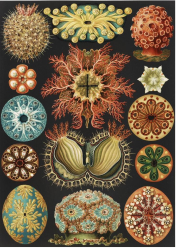
\includegraphics[width=0.5\textwidth,height=\textheight]{images/animals-pdftocairo.svg}
\caption{SVG version of the \texttt{animals}
image.}\label{fig:animals-pdftocairo-svg}
}
\end{figure}

The images appear the same visually and do not seem to have lost
definition in the conversion from the original JPEG through the two
vector formats.

Let us collate and view the file sizes of all the \texttt{animals}
images in the PDF and SVG formats, including those previously converted
using \texttt{convert} from \texttt{ImgeMagick}.

\begin{Shaded}
\begin{Highlighting}[]
\FunctionTok{ls} \AttributeTok{{-}Xsh}\NormalTok{ animals.jpg animals{-}}\DataTypeTok{\{I}\OperatorTok{,}\DataTypeTok{p\}}\PreprocessorTok{*}\NormalTok{.pdf animals}\PreprocessorTok{*}\NormalTok{.svg }\KeywordTok{|} \DataTypeTok{\textbackslash{}}
\FunctionTok{awk} \StringTok{\textquotesingle{}\{print $1 "\textbackslash{}t" $2\}\textquotesingle{}}
\ExtensionTok{{-}{-}{-}}
\ExtensionTok{200K}\NormalTok{    animals.jpg}
\ExtensionTok{204K}\NormalTok{    animals{-}IM.pdf}
\ExtensionTok{436K}\NormalTok{    animals{-}IM.svg}
\ExtensionTok{268K}\NormalTok{    animals{-}pdftocairo.svg}
\end{Highlighting}
\end{Shaded}

We may infer that, for conversion to SVG:

\begin{enumerate}
\item
  Direct conversion from JPEG to PDF, or from PDF to SVG, does not
  substantially degrade image quality or increase file size for visually
  rich, non-textual images like \texttt{animals}.
\item
  Direct conversion from JPEG to SVG using \texttt{convert} results in a
  much larger file size than if we converted from JPEG to PDF and used
  \texttt{pdftocairo} to convert that PDF to SVG. Two stage-conversion
  may therefore be preferable, at least in some cases.
\item
  \texttt{pdftoppm} is not set up to convert \emph{to} SVG, and hence
  cannot be used.
\end{enumerate}

\hypertarget{the-standalone-pdf2svg-utility}{%
\paragraph{\texorpdfstring{The standalone \texttt{pdf2svg}
utility}{The standalone pdf2svg utility}}\label{the-standalone-pdf2svg-utility}}

There is a utility called
\href{https://github.com/dawbarton/pdf2svg}{\texttt{pdf2svg}} that has
been available for some time now. It may be used to accomplish the same
PDF to SVG conversion as \texttt{pdftocairo}:

\begin{Shaded}
\begin{Highlighting}[]
\CommentTok{\# PDF to SVG using pdf2svg}
\ExtensionTok{pdf2svg}\NormalTok{ animals{-}IM.pdf animals{-}pdf2svg.svg}

\FunctionTok{ls} \AttributeTok{{-}Xsh}\NormalTok{ animals{-}IM.pdf animals{-}pdf2svg.svg animals{-}pdftocairo.svg }\KeywordTok{|} \DataTypeTok{\textbackslash{}}
\FunctionTok{awk} \StringTok{\textquotesingle{}\{print $1 "\textbackslash{}t" $2\}\textquotesingle{}}
\ExtensionTok{{-}{-}{-}}
\ExtensionTok{204K}\NormalTok{    animals{-}IM.pdf}
\ExtensionTok{268K}\NormalTok{    animals{-}pdf2svg.svg}
\ExtensionTok{268K}\NormalTok{    animals{-}pdftocairo.svg}
\end{Highlighting}
\end{Shaded}

The file sizes are identical to those from the \texttt{pdftocairo}
conversion. Drew Barton, the author of \texttt{pdf2svg},
\href{https://cityinthesky.co.uk/opensource/pdf2svg/}{has written}:

\begin{quote}
Note: since this utility was written, the maintainers of Poppler have
written a utility that works on the same principle: \texttt{pdftocairo}.
I recommend that you use their utility since it is better maintained
than mine.
\end{quote}

So, it appears that \texttt{pdftocairo} is sufficient for converting
from PDF to SVG.

\hypertarget{pdf-to-svg-with-the-text-only-image}{%
\subsubsection{\texorpdfstring{PDF to SVG with the \texttt{text-only}
image}{PDF to SVG with the text-only image}}\label{pdf-to-svg-with-the-text-only-image}}

We have already converted from PDF to SVG using \texttt{pdftocairo}
\protect\hyperlink{generating-an-svg-from-a-pdf}{previously}. We repeat
below the identical command used before to generate the SVG image:

\begin{Shaded}
\begin{Highlighting}[]
\ExtensionTok{pdftocairo} \AttributeTok{{-}svg}\NormalTok{ text{-}only.pdf text{-}only{-}pdftocairo.svg}

\FunctionTok{ls} \AttributeTok{{-}Xsh}\NormalTok{ text{-}only.pdf text{-}only{-}pdftocairo.svg }\KeywordTok{|} \FunctionTok{awk} \StringTok{\textquotesingle{}\{print $1 "\textbackslash{}t" $2\}\textquotesingle{}}
\ExtensionTok{{-}{-}{-}}
\ExtensionTok{16K}\NormalTok{     text{-}only.pdf}
\ExtensionTok{12K}\NormalTok{     text{-}only{-}pdftocairo.svg}
\ExtensionTok{{-}{-}{-}}
\ExtensionTok{pdfinfo}\NormalTok{ text{-}only.pdf }\KeywordTok{|} \FunctionTok{grep}\NormalTok{ pts}
\ExtensionTok{{-}{-}{-}}
\ExtensionTok{Page}\NormalTok{ size:      214.31 x 52.16 pts}
\ExtensionTok{{-}{-}{-}}
\FunctionTok{less}\NormalTok{ text{-}only{-}pdftocairo.svg }\KeywordTok{|} \FunctionTok{grep}\NormalTok{ viewBox}
\ExtensionTok{{-}{-}{-}}
\OperatorTok{\textless{}}\NormalTok{svg }\VariableTok{xmlns}\OperatorTok{=}\StringTok{"http://www.w3.org/2000/svg"} \ExtensionTok{xmlns:xlink=}\StringTok{"http://www.w3.org/1999/xlink"}\NormalTok{ width=}\StringTok{"214.31pt"}\NormalTok{ height=}\StringTok{"52.16pt"}\NormalTok{ viewBox=}\StringTok{"0 0 214.31 52.16"}\NormalTok{ version=}\StringTok{"1.2"}\OperatorTok{\textgreater{}}
\end{Highlighting}
\end{Shaded}

The PDF \emph{page size} and the SVG \emph{viewBox} are identical at
214.31 by 52.16 pts, as we would expect. For comparison, the
\href{images/text-only.pdf}{\texttt{text-only.pdf} image} may be opened
on a separate browser tab and compared with the SVG shown in
\cref{fig:SVGfromPDFviapdftocairo}.

\begin{figure}
\hypertarget{fig:SVGfromPDFviapdftocairo}{%
\centering

\includegraphics[width=0.8\textwidth,height=\textheight]{images/text-only-pdftocairo.svg}
\caption{SVG version of \texttt{text-only} image converted from PDF by
\texttt{pdftocairo}.}\label{fig:SVGfromPDFviapdftocairo}
}
\end{figure}

\hypertarget{pdf-to-svg-to-pdf-roundtrip}{%
\paragraph{PDF to SVG to PDF
roundtrip}\label{pdf-to-svg-to-pdf-roundtrip}}

We could open up \texttt{text-only.svg} in \texttt{Inkscape} and save it
as a PDF, \texttt{text-only-inkscape.pdf} completing the round trip. Or
we could use the command line so:

\begin{Shaded}
\begin{Highlighting}[]
\ExtensionTok{inkscape}\NormalTok{ text{-}only.svg }\AttributeTok{{-}o}\NormalTok{ text{-}only{-}inkscape.pdf}

\FunctionTok{ls} \AttributeTok{{-}Xsh}\NormalTok{ text{-}only}\PreprocessorTok{*}\NormalTok{.}\DataTypeTok{\{svg}\OperatorTok{,}\DataTypeTok{pdf\}}\KeywordTok{|} \FunctionTok{awk} \StringTok{\textquotesingle{}\{print $1 "\textbackslash{}t" $2\}\textquotesingle{}}
\ExtensionTok{{-}{-}{-}}
\ExtensionTok{8.0K}\NormalTok{    text{-}only{-}inkscape.pdf}
\ExtensionTok{16K}\NormalTok{     text{-}only.pdf}
\ExtensionTok{12K}\NormalTok{     text{-}only.svg}
\end{Highlighting}
\end{Shaded}

What exactly has been gained or lost in this round trip is a little too
recondite to consider here, and covers issues such as PDF version, font
embedding or its absence, default borders, etc.

\hypertarget{svg-to-pdf}{%
\subsubsection{SVG to PDF}\label{svg-to-pdf}}

When SVG is the source image, there are four routes to format
conversion:

\begin{enumerate}
\item
  \href{https://cairosvg.org/}{\texttt{cairosvg}}, which parses
  well-formed SVG files, draws them on a Cairo surface, and then uses
  \texttt{cairo} to export them to PDF,
  \href{https://techterms.com/definition/postscript}{PS}, PNG, and even
  to SVG again.
\item
  \href{https://en.wikipedia.org/wiki/Librsvg}{\texttt{rsvg-convert}},
  which is based on \texttt{librsvg} and which uses \texttt{libxml} and
  \texttt{cairo} to render and convert SVG files into other formats.
\item
  \href{https://inkscape.org/}{\texttt{inkscape}}, which opens SVG files
  natively and can export them as a PDF, PNG, etc.
\item
  \href{https://imagemagick.org/script/convert.php}{\texttt{convert}},
  which can convert an SVG to PDF and also to any raster format like
  PNG.
\end{enumerate}

\hypertarget{svg-to-pdftext-only}{%
\subsubsection{\texorpdfstring{SVG to
PDF:\texttt{text-only}}{SVG to PDF:text-only}}\label{svg-to-pdftext-only}}

Let us use the file \texttt{text-only-pdftocairo.svg} as the input and
convert it to PDF using all four means, and compare the resulting file
sizes:

\begin{Shaded}
\begin{Highlighting}[]
\ExtensionTok{cairosvg} \AttributeTok{{-}f}\NormalTok{ pdf }\AttributeTok{{-}o}\NormalTok{ text{-}only{-}cairosvg.pdf text{-}only{-}pdftocairo.svg}

\ExtensionTok{rsvg{-}convert} \AttributeTok{{-}f}\NormalTok{ pdf }\AttributeTok{{-}o}\NormalTok{ text{-}only{-}rsvg{-}convert.pdf text{-}only{-}pdftocairo.svg}

\ExtensionTok{inkscape}\NormalTok{ text{-}only{-}pdftocairo.svg }\AttributeTok{{-}o}\NormalTok{ text{-}only{-}inkscape.pdf}

\ExtensionTok{convert}\NormalTok{ text{-}only{-}pdftocairo.svg text{-}only{-}IM.pdf}

\FunctionTok{ls} \AttributeTok{{-}Xsh}\NormalTok{ text{-}only{-}pdftocairo.svg text{-}only{-}}\DataTypeTok{\{c}\OperatorTok{,}\DataTypeTok{r}\OperatorTok{,}\DataTypeTok{i}\OperatorTok{,}\DataTypeTok{I\}}\PreprocessorTok{*}\NormalTok{.pdf }\KeywordTok{|} \DataTypeTok{\textbackslash{}}
\FunctionTok{awk} \StringTok{\textquotesingle{}\{print $1 "\textbackslash{}t" $2\}\textquotesingle{}}
\ExtensionTok{{-}{-}{-}}
\ExtensionTok{8.0K}\NormalTok{    text{-}only{-}cairosvg.pdf}
\ExtensionTok{8.0K}\NormalTok{    text{-}only{-}IM.pdf}
\ExtensionTok{8.0K}\NormalTok{    text{-}only{-}inkscape.pdf}
\ExtensionTok{8.0K}\NormalTok{    text{-}only{-}rsvg{-}convert.pdf}
\ExtensionTok{12K}\NormalTok{     text{-}only{-}pdftocairo.svg}
\end{Highlighting}
\end{Shaded}

The PDF file sizes are the same from the different conversion methods.
Since the \emph{viewBox} of the input SVG is the same and the file
content is the same, the PDF \emph{Page size} is the same for all PDFs.

Comparison with the original file
\href{images/text-only.pdf}{\texttt{text-only.pdf}} shows the following
differences:

\begin{enumerate}
\def\labelenumi{\alph{enumi}.}
\item
  The three files \href{attach}{\texttt{text-only-cairosvg.pdf}},
  \href{images/text-only-inkscape.pdf}{\texttt{text-only-inkscape.pdf}},
  and
  \href{images/text-only-rsvg-convert.pdf}{\texttt{text-only-rsvg-convert.pdf}}
  all show a white border on three sides of the converted PDF file.
  Zooming shows no degradation in image quality.
\item
  The fourth file,
  \href{images/text-only-IM.pdf}{\texttt{text-only-IM.pdf}} obviously
  went through an intermediate raster phase and shows blockiness when
  zoomed. Direct conversion from SVG to PDF vis
  \texttt{ImageMagick\ convert} should be avoided.
\end{enumerate}

\hypertarget{svg-to-pdf-animals}{%
\subsubsection{\texorpdfstring{SVG to PDF:
\texttt{animals}}{SVG to PDF: animals}}\label{svg-to-pdf-animals}}

We use the file \texttt{animals-pdftocairo.svg} as source to convert to
PDF and list the commands and file sizes below:

\begin{Shaded}
\begin{Highlighting}[]
\ExtensionTok{cairosvg} \AttributeTok{{-}f}\NormalTok{ pdf }\AttributeTok{{-}o}\NormalTok{ animals{-}cairosvg.pdf animals{-}pdftocairo.svg}

\ExtensionTok{rsvg{-}convert} \AttributeTok{{-}f}\NormalTok{ pdf }\AttributeTok{{-}o}\NormalTok{ animals{-}rsvg{-}convert.pdf animals{-}pdftocairo.svg}

\ExtensionTok{inkscape}\NormalTok{ animals{-}pdftocairo.svg }\AttributeTok{{-}o}\NormalTok{ animals{-}inkscape.pdf}

\ExtensionTok{convert}\NormalTok{ animals{-}pdftocairo.svg animals{-}from{-}svg{-}IM.pdf}

\FunctionTok{ls} \AttributeTok{{-}Xsh}\NormalTok{ animals{-}pdftocairo.svg animals{-}}\DataTypeTok{\{c}\OperatorTok{,}\DataTypeTok{r}\OperatorTok{,}\DataTypeTok{i}\OperatorTok{,}\DataTypeTok{f\}}\PreprocessorTok{*}\NormalTok{.pdf }\KeywordTok{|} \DataTypeTok{\textbackslash{}}
\FunctionTok{awk} \StringTok{\textquotesingle{}\{print $1 "\textbackslash{}t" $2\}\textquotesingle{}}
\ExtensionTok{{-}{-}{-}}
\ExtensionTok{1.9M}\NormalTok{    animals{-}cairosvg.pdf}
\ExtensionTok{200K}\NormalTok{    animals{-}from{-}svg{-}IM.pdf}
\ExtensionTok{204K}\NormalTok{    animals{-}inkscape.pdf}
\ExtensionTok{1.9M}\NormalTok{    animals{-}rsvg{-}convert.pdf}
\ExtensionTok{268K}\NormalTok{    animals{-}pdftocairo.svg}
\end{Highlighting}
\end{Shaded}

The page sizes are similar but the file sizes differ by an order of
magnitude for the different PDFs. Those output by the \texttt{cairo}
library are almost ten times larger than those put out by
\texttt{ImageMagick} and \texttt{Inkscape}.

You may compare the appearance of all four images by clicking on
separate browser tabs for these four images and zooming in to see
details:

\begin{itemize}
\tightlist
\item
  \href{images/animals-cairosvg.pdf}{\texttt{animals-cairosvg.pdf}}
\item
  \href{images/animals-from-svg-IM.pdf}{\texttt{animals-from-svg-IM.pdf}}
\item
  \href{images/animals-inkscape.pdf}{\texttt{animals-inkscape.pdf}}
\item
  \href{images/animals-rsvg-convert.pdf}{\texttt{animals-rsvg-convert.pdf}}
\end{itemize}

The image \texttt{animals-from-svg-IM.pdf} is pixellated on zooming in
and we should avoid this conversion for images with fine detail. The two
images weighing in at a file size of 1.9M exhibit detail commensurate
with their heft. The image \texttt{animals-inkscape.pdf} is the
preferred option as it balances good rendition of detail with a
tractable file size.

\hypertarget{summary}{%
\subsection{Summary}\label{summary}}

\begin{enumerate}
\item
  \texttt{convert} from \texttt{ImageMagick} is the tool of choice for
  converting from any raster format to another raster format or to PDF
  or SVG.
\item
  When we start out with PDF as the source image format, and the
  destination format is either a raster format or SVG, the tool of
  choice is \texttt{pdftocairo} from the \texttt{poppler} utilities.
\item
  When the source format is SVG and the destination format is either PDF
  or a raster format, the tools of choice are either \texttt{cairosvg}
  or \texttt{inkscape} depending on image content.
\end{enumerate}

\cref{tbl:formats} summarizes this information, which is current at the
time of writing, but could change as the image utilities landscape
changes with time.

\hypertarget{tbl:formats}{}
\begin{longtable}[]{@{}ll@{}}
\caption{\label{tbl:formats}Tools for image format
conversions.}\tabularnewline
\toprule
Conversion Type & Tool \\
\midrule
\endfirsthead
\toprule
Conversion Type & Tool \\
\midrule
\endhead
raster to raster & \texttt{convert} \\
raster to PDF & \texttt{convert} \\
raster to SVG & \texttt{convert} \\
PDF to raster & \texttt{pdftoppm} \\
SVG to raster & \texttt{cairosvg} \\
PDF to SVG & \texttt{pdftocairo} \\
SVG to PDF & \texttt{inkscape} \\
\bottomrule
\end{longtable}

\hypertarget{appendix-security-vulnerabilities-in-imagemagick}{%
\subsection{\texorpdfstring{Appendix: Security vulnerabilities in
\texttt{ImageMagick}}{Appendix: Security vulnerabilities in ImageMagick}}\label{appendix-security-vulnerabilities-in-imagemagick}}

Great power exacts a commensurate price. \texttt{ImageMagick}'s great
power and ease of use does come at a great price: vulnerability to
exploits by malicious remote actors.

\texttt{ImageMagick} uses external libraries or \emph{backend tools}
which are called via \texttt{system()} commands in accordance with
\emph{delegated} command strings specified in a configuration file
called \texttt{policy.xml}.

In April 2016, it was reported that because of insufficient validation
of delegated command strings, it was possible for someone to execute
malicious code remotely, to the detriment of the unwitting user of
\texttt{ImageMagick}. This was revealed at a website, interestingly
named \href{https://imagetragick.com/}{ImageTragick} to attract
sufficient attention and remedial action to the discovered bug
\protect\hyperlink{ref-imagetragick2016}{{[}7{]}}.

In November 2020,
\href{https://portswigger.net/daily-swig/imagemagick-pdf-parsing-flaw-allowed-attacker-to-execute-shell-commands-via-maliciously-crafted-image}{another
security vulnerability was discovered}
\protect\hyperlink{ref-leyden2020}{{[}8{]}}. It was
\href{https://insert-script.blogspot.com/2020/11/imagemagick-shell-injection-via-pdf.html}{reported
and promptly patched} by the \texttt{ImageMagick} maintainers
\protect\hyperlink{ref-infuhr2020}{{[}9{]}}.

Recent versions of the \texttt{ImageMagick} suite, bundled with major
distributions, should have correctly configured \texttt{policy.xml}
files that will block known exploits.
\href{https://www.techopedia.com/definition/25266/sandboxing}{Sandboxing}
is another technique to quarantine the system from possible
vulnerabilities. Above all, it is vital to keep system and application
software up to date to avail of evolutions in performance and security.

\hypertarget{feedback}{%
\subsection{Feedback}\label{feedback}}

Please \href{mailto:feedback.swanlotus@gmail.com}{email me} your
comments and corrections.

\noindent A PDF version of this article is
\href{image-format-conversions.pdf}{available for download here.}

\hypertarget{bibliography}{%
\section*{References}\label{bibliography}}
\addcontentsline{toc}{section}{References}

\hypertarget{refs}{}
\begin{CSLReferences}{0}{0}
\leavevmode\vadjust pre{\hypertarget{ref-gabriel2017}{}}%
\CSLLeftMargin{{[}1{]} }
\CSLRightInline{S. Gabriel, {`{Designer's guide to DPI}'}, 15-May-2015.
{[}Online{]}. Available:
\url{https://sebastien-gabriel.com/designers-guide-to-dpi/}.
{[}Accessed: 27-Mar-2021{]}}

\leavevmode\vadjust pre{\hypertarget{ref-imagemagicksource}{}}%
\CSLLeftMargin{{[}2{]} }
\CSLRightInline{ImageMagick Studio LLC, {`ImageMagick 7'}. {[}Online{]}.
Available: \url{https://github.com/ImageMagick/ImageMagick}.
{[}Accessed: 08-Mar-2021{]}}

\leavevmode\vadjust pre{\hypertarget{ref-imcli}{}}%
\CSLLeftMargin{{[}3{]} }
\CSLRightInline{{`{ImageMagick---Command-line Processing}. {Anatomy of
the Command-line}'}. {[}Online{]}. Available:
\url{https://imagemagick.org/script/command-line-processing.php}.
{[}Accessed: 12-Mar-2021{]}}

\leavevmode\vadjust pre{\hypertarget{ref-newton2015}{}}%
\CSLLeftMargin{{[}4{]} }
\CSLRightInline{D. Newton, {`{Efficient Image Resizing With
ImageMagick---Smashing Magazine}'}, 25-Jun-2015. {[}Online{]}.
Available:
\url{https://www.smashingmagazine.com/2015/06/efficient-image-resizing-with-imagemagick/}.
{[}Accessed: 11-Mar-2021{]}}

\leavevmode\vadjust pre{\hypertarget{ref-setchell2014}{}}%
\CSLLeftMargin{{[}5{]} }
\CSLRightInline{M. Setchell, {`{ImageMagick: Lossless max compression
for PNG?---Stack Overflow}'}, 03-Dec-2014. {[}Online{]}. Available:
\url{https://stackoverflow.com/questions/27267073/imagemagick-lossless-max-compression-for-png/27269260\#27269260}.
{[}Accessed: 12-Mar-2021{]}}

\leavevmode\vadjust pre{\hypertarget{ref-oreilly2019}{}}%
\CSLLeftMargin{{[}6{]} }
\CSLRightInline{A. Bellamy-Royds, K. Cagle, and D. Storey, {`{Units for
Measurements Reference --- Using SVG with CSS3 and HTML5---Supplementary
Material}'}, 05-Oct-2019. {[}Online{]}. Available:
\url{https://oreillymedia.github.io/Using_SVG/guide/units.html}.
{[}Accessed: 20-Mar-2021{]}}

\leavevmode\vadjust pre{\hypertarget{ref-imagetragick2016}{}}%
\CSLLeftMargin{{[}7{]} }
\CSLRightInline{---, {`ImageMagick is on fire --- CVE-2016--3714'},
12-May-2016. {[}Online{]}. Available: \url{https://imagetragick.com/}.
{[}Accessed: 08-Mar-2021{]}}

\leavevmode\vadjust pre{\hypertarget{ref-leyden2020}{}}%
\CSLLeftMargin{{[}8{]} }
\CSLRightInline{J. Leyden, {`ImageMagick PDF-parsing flaw allowed
attacker to execute shell commands via maliciously crafted image'},
23-Nov-2020. {[}Online{]}. Available:
\url{https://portswigger.net/daily-swig/imagemagick-pdf-parsing-flaw-allowed-attacker-to-execute-shell-commands-via-maliciously-crafted-image}.
{[}Accessed: 08-Mar-2021{]}}

\leavevmode\vadjust pre{\hypertarget{ref-infuhr2020}{}}%
\CSLLeftMargin{{[}9{]} }
\CSLRightInline{A. Inführ, {`{ImageMagick - Shell injection via PDF
password}'}, 21-Nov-2020. {[}Online{]}. Available:
\url{https://insert-script.blogspot.com/2020/11/imagemagick-shell-injection-via-pdf.html}.
{[}Accessed: 08-Mar-2021{]}}

\end{CSLReferences}



\end{document}
